\documentclass[preprint]{aastex}
\shorttitle{PAPER 64-Station Results}
\shortauthors{Parsons, et al.}

\usepackage{amsmath}
\usepackage{graphicx}
\usepackage[figuresright]{rotating}
%\usepackage{rotating}
\usepackage{natbib}
%\usepackage{pdflscape}
\usepackage{lscape}
\citestyle{aa}

\begin{document}
\title{PAPER-64: Southern-Hemisphere Source Spectra}

\author{Aaron R. Parsons}

\begin{abstract}
\end{abstract}

\section{Introduction}

Numerous radio telescopes are now exploring the prospects for
using measurements of highly redshifted 21cm emission to inform our understanding
of cosmic reionization. 
These include telescopes aiming to measure the global temperature change of 
21cm emission during the Epoch of Reionization (EoR), such as
the Compact Reionization Experiment (CoRE) and
the Experiment to Detect the Global EoR Signature (EDGES; \citealt{bowman_rogers2010}),
and interferometers aiming to measure the power spectrum of 21-cm EoR emission, such as
the Giant Metre-wave Radio Telescope (GMRT;
\citealt{pen_et_al2009})\footnote{\url{http://gmrt.ncra.tifr.res.in/}},
the LOw Frequency ARray (LOFAR; \citealt{rottgering_et_al2006})\footnote{\url{http://www.lofar.org/}},
the Murchison Widefield Array (MWA; \citealt{lonsdale_et_al2009})\footnote{\url{http://www.mwatelescope.org/}}, 
and 
the Donald C. Backer Precision Array for Probing the Epoch of Reionization (PAPER;
\citealt{parsons_et_al2010})\footnote{\url{http://eor.berkeley.edu/}}.

As such, there has been a renewed interest in the spectral and spatial variation of 
foreground emission in the 100--200 MHz frequency band that covers
the $z=6$--13 redshift range expected to encompass reionization
\citep{furlanetto_et_al2006}.
In particular, the spectral properties of extra-galactic point-sources are important
both because they are valuable calibration references
and because they are strong foreground emitters that must be removed from 21-cm EoR measurements.
With the sparse availability of measured foreground properties in the
100--200-MHz frequency band over large areas of the sky \citep{deolivieracosta_et_al2008}, continued 
foreground characterization is a
vital step en route to any 21-cm EoR detection.

%Since the 
%first-generation radio telescopes 
%are strongly influenced by the estimated angular power-spectra and
%frequency-dependence of foregrounds \citep{wang_et_al2006,bowman_et_al2009,parsons_et_al2011}.

In this paper, we report source spectra derived from PAPER observations.
PAPER is a dedicated experiment 
that employs non-tracking, dual-polarization dipole antennas 
tuned for efficient operation over a 120--170-MHz band.
PAPER employs two distinct deployments. PAPER Green Bank, at the NRAO site 
near Green Bank, WV,
is used primarily for engineering investigations and field testing.  PAPER South Africa
(PSA) is used primarily for science observations, and is data from this deployment
on which this paper is based.  PSA is located in the Karoo desert
on the Square Kilometer Array
South Africa (SKA-SA) reserve, somewhat near the small town of Carnarvon.
The PSA array has grown from 16 elements deployed in early 2009 to the
64-element array currently in use.

This paper is structured as follows:
in \S\ref{sec:} we XXX...

with primary beams that illuminate
a large ($\sim$1 sr) field of view.

\section{Observations}
\label{sec:observations}

\begin{figure*}\centering
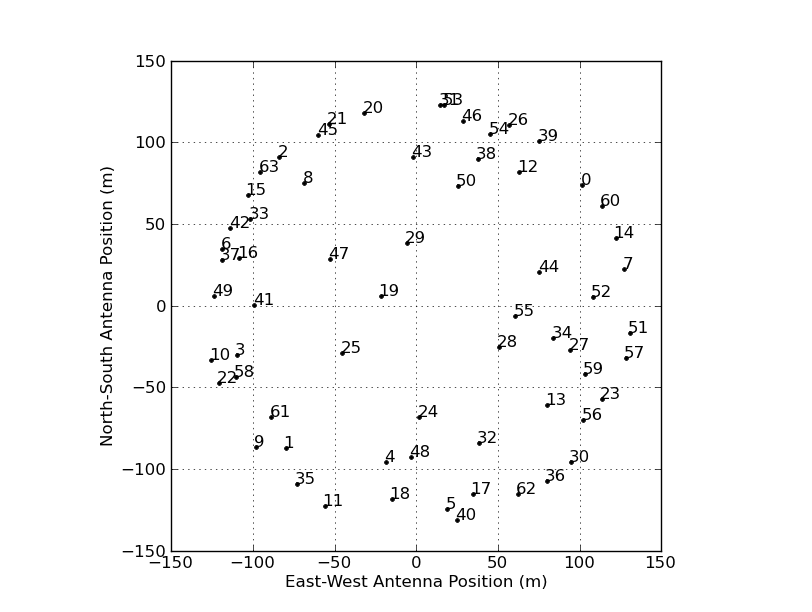
\includegraphics[width=0.85\columnwidth]{plots/antpos.png}
\caption{The 64-antenna, minimum-redundancy array configuration used by the PAPER deployment
in the Karoo Radio Observatory site in South Africa for these observations.
}\label{fig:antpos}
\end{figure*}

Measurements are derived from observations using only the east-west dipole arms of 64 PAPER antennas 
deployed in the Karoo Radio Observatory site in South Africa (see Figure \ref{fig:antpos}).  
A 100-MHz band from 100-200MHz was
correlated with 1024 frequency channels and integrated for 10.7 seconds before visibilities were stored.
Source spectra measured over the course of a 24-hour observing run on July 4, 2011, running
from JD2455747.15 to JD2455748.12.
Two antennas (\#40,\#55) were omitted owing to malfunctioning signal path, leaving 62 remaining antennas
used in the observations.

Quantization gain through the correlator was linearized \citep{parsons_et_al2008}.
Removed RFI by flagging samples in each frequency channel versus time that exceed the mean amplitude by 4-sigma
after performing a time derivative.  Also flagged samples in each integrated spectrum that exceeded the
mean amplitude across the spectrum by 6-sigma after performing a frequency derivative.  For efficiency, flagging
was derived using only the subset of baselines involving a fiducial antenna.
Frequencies below 120 MHz and above 180 MHz were also flagged, owing to roll-off of analog response.
After RFI flagging, frequency channel resolution was decreased by a factor of four by summing channels.
Finally, measurements of ambient temperature versus time near the balun amplifier of a fiducial antenna and near
receiver amplifiers were used to divide out the predicted gain variation versus temperature that these amplifiers
are known to exhibit.  A predicted gain profile was drived using coefficients characterized in 
laboratory measurements \citep{parashare_bradley2009} and
confirmed in field measurements \citep{pober_et_al2011} of $H_{\rm balun}=-0.024$ dB/K, $H_{\rm recvr}=-0.045$
dB/K, and $H_{\rm cable}=-0.018$ dB/K for 150m-long cables.  Because cable temperatures were not measured
during these observations, the cable temperature was assumed to be the same as the measured balun temperature.

\begin{figure*}\centering
\includegraphics[width=0.85\columnwidth]{plots/tempgain.png}
\caption{Upper panel: ambient temperatures measured near various components with temperature-dependent
gains in the PAPER analog signal chain versus time offset from JD2455747.0. Lower panel: the 
predicted multiplicative gain that is corrected for using the temperature curves and the gain coefficients
listed in \S\ref{sec:observations}.
}\label{fig:tempgain}
\end{figure*}

Phase calibration performed using the central components of Centaurus A, Fornax A, and Pictor A.
The overall gain and bandpass were calibrated to J2214-170 listed by Helmboldt et al. (2006).

As the sky drifts through the primary beam of PAPER antennas, widely
separated points will be observed with substantially different gains and
so will require different data weightings to optimize SNR.

Drift-scan observations of sources were divided by the calibrated beam response in the
direction of the source as a function of time.  Spectra were calculated by averaging over
time, weighting data at each time step by the square of the 150-MHz beam response in the source direction.
Since noise and systematics relating to source observations are expected to be approximately constant
versus time, while source amplitude is proportional to beam response, this weighting 
is an effective approximation of inverse-variance weighting \citep{pober_et_al2011}.

After measuring their spectra, point-source models of the brightest sources (Centaurus A, Fornax A, 
Pictor A, Sun, Virgo A,
and Cygnus A) were subtracted from visibilities, and bright sources at low altitudes (Sun, Virgo A,
and Cygnus A) where antenna response models are less reliable were further surpressed with DDR 
filters \citep{parsons_backer2009}.  Remaining source used these filtered/subtracted visibilities
for characterizing their spectra in order to reduce sidelobe contamination.

Finally, data from all baselines longer than 20 wavelengths were phased toward each source
and summed using natural weighting to produce a beam tracking that source, yielding a measured
source spectrum for each time integation.

\begin{figure*}\centering
%\includegraphics[width=0.85\columnwidth]{plots/skymap.png}
\caption{
}\label{fig:skymap}
\end{figure*}

\begin{figure*}\centering
%\includegraphics[width=0.85\columnwidth]{plots/skymap_eq.png}
\caption{
}\label{fig:skymap_eq}
\end{figure*}



\section{Target Selection}
\label{sec:target_selection}

A first set of source targets were selected from the Helmboldt \citep{helmboldt_et_al2008}, Culgoora \citep{slee1995}, and
Mauritius Radio Telescope \citep{golap_et_al1998} catalogs, restricted to sources with fluxes at 150 MHz 
exceeding 5 Jys and source declination 
falling within $\pm20^\circ$ of the -30:43 latitude
of the PAPER array.  Sources within $\pm10^\circ$ of the galactic plane were also excluded, as were
sources near Centaurus A ($\pm5^\circ$ in declination, $\pm2.5^\circ$ in right-ascension).


\section{Discussion}

\begin{figure*}\centering
\includegraphics[width=0.85\columnwidth]{plots/catcompare.png}
\caption{A comparison of catalogued flux-density extrapolated to 150 MHz (horizontal axis) versus 
measured flux-density (vertical axis) for various catalogs.
}\label{fig:catcompare}
\end{figure*}

A comparison of measured source fluxes at 150 MHz and catalog values extrapolate to that frequency
is illustrated in Figure \ref{fig:catcompare}.
Comparison with PSA32 catalog \citep{jacobs_et_al2011}.

\begin{figure*}\centering
\includegraphics[width=0.85\columnwidth]{plots/numcounts.png}
\caption{Number counts (vertical axis) versus flux-density at 150 MHz (horizontal axis), normalized
to the angular area of XXX sr surveyed for this catalog.  Source count statistics from this
catalog (black crosses) are compared with pixel statistics derived from imaging various regions:
the entire sky below $\delta=0^\circ$ (green), the galactic plane $\pm10^\circ$ latitude below
$\delta=0^\circ$ (magenta), the region surveyed for this catalog (black, as described 
in \S\ref{sec:target_selection}), and the region outside the galactic plane below $\delta=0^\circ$
that was not included in this survey (cyan).
}\label{fig:numcounts}
\end{figure*}

Source-count statistics versus flux density for this catalog are shown in 
Figure \ref{fig:numcounts}, along with comparisons to pixel-count statistics for an all-sky map
generated from the same data (see Figure \ref{fig:skymap}).  In addition to justifying the
selection of angular area described in \S\ref{sec:target_selection} for producing this 
catalog on the basis of disparate source-count statistics, Figure \ref{fig:numcounts} 
provides context for ruling out selection bias and target ambiguity arising from confusion.
The chosen selection threshold of 5 Jy lies a factor of five higher than the $\sim$1-Jy threshold
at which the number density of source fluxes departs from a power law.

\section{Conclusion}

This cataloging work is part of a broader initiative in foreground characterization 
in the 100-200MHz frequency band.  Future work in this area 
will include updating
and expanding previous source catalogs, measuring the effects of
ionospheric refraction on source removal, mapping galactic synchrotron
emission, using rotation measure synthesis to determine the frequency
dependence of synchrotron polarization structure, and directly
measuring the magnitude of emission and absorption from radio
recombination lines in galactic emission.  The global sky model
resulting from this work will be used to remove foreground emission
from 21cm EoR experiments, and to estimate residual systematic biases in power
spectrum measurements.  

Meanwhile, work is underway to
expand PSA to 128 antennas in the near future.

The modest size of the ground-screen reflecting structure and the fact
that PAPER employs rugged above-ground cables to carry signals from the antenna
elements to a central location for correlation allow PAPER antennas to be
moved relativlty easily.
PAPER is in a unique position to use the mobility of its antennas to
explore different configurations.  Current PAPER observing activities aim to explore
the feasibility of tuning array sensitivity relative to foreground
brightness \citep{parsons_et_al2011}.  

Research
activities in the near term will focus on improving the
characterization of the PAPER primary beam and mapping foreground
emission with the goal of establishing a global sky model for removing
foreground emission from PAPER data and estimating residual systematic
biases in power spectrum measurements.  Results from foreground
characterization will also be directly applicable to other
reionization efforts, providing a valuable point of contact with other
HERA progenitors and with the global reionization community.

An important step in route to obtaining a high-sensitivity power spectrum
measurement is to direct the sensitivity of the PAPER-128 array in a
low-redundancy configuration toward improving the global sky model.
The foreground model established in this stage of PAPER observing will
be generally useful for all reionization experiments operating at
these frequencies.  These observing activities will also be useful
within PAPER for re-establishing calibration parameters, verifying
instrumental performance, and removing foregrounds from power-spectrum
detection observations.

Results from this work will be disseminated as
source catalogs and all-sky maps in the HEALPix FITS format \citep{gorski_et_al2006} as a
resource for the global reionization community.

\section{Acknowledgment}

We would like to thank SKA-SA for the site infrastructure, maintanence, and observing support
that has made this work possible.

\begin{table}[ht]
\caption{Measured Source Parameters}
\begin{tabular}{l|lrrr||l|lrrr}
\hline
Name & RA & DEC & $f_{150}$ & $\alpha$ & Name & RA & DEC & $f_{150}$ & $\alpha$
\\
\hline
  0000-362 &  0:03 & -35:57 &   13.1 & -0.54 &   0057-180 &  1:00 & -17:49 &    7.0 & -0.29 \\
 J0003-173 &  0:03 & -17:27 &   24.1 & -0.86 &   0100-221 &  1:02 & -21:52 &   14.7 & -1.03 \\
MRTJ0003-3059 &  0:03 & -30:59 &    8.7 & +0.19 &   0100-278 &  1:02 & -27:32 &    9.9 & -0.45 \\
MRTJ0006-4234 &  0:06 & -42:34 &   21.2 & +0.16 &   0101-416 &  1:03 & -41:20 &    9.2 & +0.12 \\
MRTJ0009-4503 &  0:09 & -45:03 &    8.0 & +0.12 &   0102-384 &  1:05 & -38:10 &   12.6 & -0.38 \\
MRTJ0010-4339 &  0:10 & -43:39 &    9.2 & +0.19 &   0103-453 &  1:05 & -45:05 &   45.7 & -0.01 \\
MRTJ0010-4423 &  0:10 & -44:23 &   32.9 & +0.06 &  J0108-160 &  1:08 & -16:04 &   59.1 & -1.09 \\
MRTJ0012-3322 &  0:12 & -33:22 &   10.4 & +0.16 &   0112-445 &  1:14 & -44:18 &    8.9 & +0.27 \\
  0012-383 &  0:15 & -38:05 &   18.2 & -0.16 &   0114-476 &  1:16 & -47:24 &   38.1 & -0.26 \\
  0013-147 &  0:16 & -14:30 &    6.9 & -0.97 &   0114-211 &  1:16 & -20:52 &   15.5 & +0.17 \\
MRTJ0016-3827 &  0:16 & -38:27 &    8.5 & -0.30 &   0116-413 &  1:18 & -41:02 &    6.9 & -0.46 \\
 J0019-124 &  0:18 & -12:42 &   12.3 & -0.32 &  J0120-152 &  1:20 & -15:20 &   37.8 & -0.85 \\
MRTJ0020-4847 &  0:20 & -48:47 &    8.4 & +0.11 &   0119-377 &  1:22 & -37:30 &   15.2 & -0.27 \\
MRTJ0020-2015 &  0:20 & -20:15 &    5.5 & -0.48 &   0122-255 &  1:24 & -25:17 &    9.3 & -0.32 \\
MRTJ0021-1910 &  0:21 & -19:10 &    6.0 & -0.36 &   0124-409 &  1:26 & -40:41 &   12.9 & +0.68 \\
MRTJ0021-4657 &  0:21 & -46:57 &   11.1 & -0.54 &   0124-414 &  1:27 & -41:12 &   18.3 & +0.00 \\
  0020-253 &  0:23 & -25:02 &   12.0 & -0.10 &  J0128-140 &  1:27 & -14:02 &   29.2 & -1.23 \\
 J0025-293 &  0:24 & -29:28 &   32.4 & -0.20 &   0125-438 &  1:27 & -43:35 &    8.4 & +0.25 \\
  0023-333 &  0:25 & -33:03 &   14.0 & -0.20 &  J0130-261 &  1:30 & -26:10 &   27.8 & -0.81 \\
  0023-263 &  0:25 & -26:02 &   24.5 & +0.41 &   0131-450 &  1:33 & -44:44 &   20.6 & -0.01 \\
MRTJ0026-4918 &  0:26 & -49:18 &    7.3 & +0.79 &   0131-367 &  1:33 & -36:29 &   49.1 & -0.29 \\
  0024-372 &  0:26 & -36:56 &    7.0 & -0.38 &   0139-273 &  1:41 & -27:06 &   12.1 & -0.06 \\
MRTJ0028-4157 &  0:28 & -41:57 &    8.4 & +0.09 &  J0142-163 &  1:42 & -16:28 &   33.1 & -1.56 \\
MRTJ0030-5018 &  0:30 & -50:18 &   10.4 & +0.35 &   0141-439 &  1:43 & -43:42 &    6.1 & -0.88 \\
 J0035-200 &  0:35 & -20:03 &   23.7 & -0.54 &   0144-374 &  1:46 & -37:11 &    9.4 & +0.41 \\
MRTJ0036-4903 &  0:36 & -49:03 &    6.9 & -0.58 &   0148-297 &  1:50 & -29:32 &   25.4 & -0.50 \\
  0034-377 &  0:36 & -37:28 &    7.5 & -0.58 &   0149-394 &  1:51 & -39:10 &    7.2 & -0.03 \\
MRTJ0038-3859 &  0:38 & -39:00 &   23.8 & -0.35 &   0149-299 &  1:52 & -29:42 &   10.3 & -0.45 \\
  0039-445 &  0:42 & -44:14 &   44.2 & +0.18 &   0152-437 &  1:54 & -43:27 &   10.5 & -0.09 \\
  0042-357 &  0:44 & -35:30 &   14.9 & +0.30 &  J0200-305 &  2:00 & -30:53 &   35.8 & -0.22 \\
  0043-424 &  0:46 & -42:07 &   73.7 & +0.22 &   0159-117 &  2:01 & -11:32 &    4.2 & -2.30 \\
  0045-255 &  0:47 & -25:17 &   24.6 & -0.24 &   0201-441 &  2:03 & -43:51 &   21.4 & +0.69 \\
  0048-447 &  0:50 & -44:28 &   23.6 & +0.01 &   0202-182 &  2:05 & -18:01 &    6.8 & -0.83 \\
  0049-433 &  0:52 & -43:06 &   32.7 & +0.20 &   0204-378 &  2:06 & -37:38 &    8.5 & -0.46 \\
 J0059-170 &  0:59 & -17:00 &   30.5 & -1.26 &   0207-112 &  2:10 & -11:00 &    6.3 & -0.85 \\
\hline
\end{tabular}
\end{table}

\begin{table}[ht]
\caption{Measured Source Parameters}
\begin{tabular}{l|lrrr||l|lrrr}
\hline
Name & RA & DEC & $f_{150}$ & $\alpha$ & Name & RA & DEC & $f_{150}$ & $\alpha$
\\
\hline
  0211-344 &  2:13 & -34:13 &    9.6 & -0.33 &   0328-370 &  3:30 & -36:53 &   15.7 & -0.43 \\
 J0216-126 &  2:15 & -12:59 &   52.4 & -1.25 &   0332-391 &  3:33 & -38:58 &   16.4 & +0.47 \\
  0213-134 &  2:15 & -13:15 &    5.4 & -0.93 &   0335-415 &  3:37 & -41:22 &   18.0 & -0.16 \\
  0214-480 &  2:16 & -47:47 &   23.4 & +0.11 &   0336-355 &  3:38 & -35:23 &   16.8 & -1.32 \\
  0216-250 &  2:18 & -24:48 &   11.2 & -0.73 &   0338-404 &  3:39 & -40:18 &   18.6 & +0.11 \\
  0216-366 &  2:19 & -36:25 &   17.1 & -0.64 &   0340-372 &  3:42 & -37:02 &   12.4 & -0.79 \\
  0217-369 &  2:19 & -36:43 &    9.0 & +0.12 &   0344-345 &  3:46 & -34:22 &   26.3 & -0.09 \\
  0218-387 &  2:20 & -38:33 &   11.0 & -0.91 &  J0351-143 &  3:51 & -14:29 &   67.1 & -1.56 \\
  0220-422 &  2:22 & -41:59 &   16.1 & -0.20 &   0349-278 &  3:51 & -27:44 &   37.8 & -0.66 \\
  0221-285 &  2:23 & -28:19 &   12.5 & -0.64 &   0354-485 &  3:55 & -48:23 &   16.1 & +0.01 \\
  0222-234 &  2:25 & -23:12 &   11.8 & -0.68 &   0358-371 &  3:59 & -37:00 &   15.8 & -0.33 \\
  0225-308 &  2:27 & -30:38 &    9.0 & +0.18 &  J0400-161 &  4:00 & -16:10 &   39.4 & -1.75 \\
  0228-399 &  2:30 & -39:44 &   10.9 & -0.56 &   0403-132 &  4:05 & -13:08 &    7.2 & -2.01 \\
  0231-235 &  2:33 & -23:21 &   12.6 & +0.01 &  J0408-121 &  4:07 & -12:11 &   25.7 & -1.01 \\
 J0238-193 &  2:37 & -19:32 &   37.5 & -0.49 &   0406-311 &  4:08 & -31:01 &    6.1 & +0.06 \\
  0240-422 &  2:42 & -42:01 &   17.8 & +0.14 &  J0409-242 &  4:08 & -24:18 &   25.0 & -1.18 \\
  0244-452 &  2:45 & -44:59 &   12.6 & -0.46 &   0411-346 &  4:13 & -34:30 &   11.9 & -0.76 \\
  0245-297 &  2:47 & -29:30 &    6.6 & -0.25 &   0413-425 &  4:15 & -42:24 &    8.2 & -1.07 \\
  0252-418 &  2:53 & -41:41 &    8.1 & +0.35 &  J0415-293 &  4:15 & -29:29 &   13.3 & -0.09 \\
 J0256-232 &  2:56 & -23:24 &   25.6 & -1.12 &  J0416-206 &  4:16 & -20:56 &   18.4 & -0.25 \\
  0257-398 &  2:59 & -39:41 &    5.9 & -1.10 &   0418-399 &  4:19 & -39:50 &    9.8 & +0.81 \\
  0302-361 &  3:04 & -35:54 &    9.3 & +0.09 &   0420-264 &  4:22 & -26:17 &    8.3 & -1.15 \\
  0304-122 &  3:06 & -12:06 &    6.2 & +0.38 &   0421-341 &  4:23 & -34:02 &    8.8 & -0.69 \\
  0305-226 &  3:07 & -22:25 &   11.9 & -0.34 &   0427-366 &  4:29 & -36:30 &   28.0 & -0.25 \\
 J0313-145 &  3:12 & -14:49 &   19.9 & -0.91 &   0431-300 &  4:32 & -29:57 &   10.7 & -0.66 \\
  0313-271 &  3:16 & -26:58 &    8.4 & -1.47 &   0431-133 &  4:33 & -13:15 &    7.0 & -3.16 \\
  0314-440 &  3:16 & -43:51 &   10.2 & -1.44 &   0435-300 &  4:37 & -29:55 &    7.6 & +0.00 \\
  0315-146 &  3:17 & -14:30 &    5.1 & -2.44 &   0438-436 &  4:40 & -43:33 &   13.8 & +1.65 \\
  0316-444 &  3:17 & -44:14 &   12.6 & -0.57 &  J0445-281 &  4:44 & -28:09 &   73.5 & -0.41 \\
  0319-453 &  3:21 & -45:10 &   37.2 & +0.00 &   0446-206 &  4:48 & -20:32 &    8.0 & -1.79 \\
  0320-389 &  3:22 & -38:47 &    6.4 & +0.79 &  J0455-301 &  4:55 & -30:06 &   41.0 & -0.60 \\
       for &  3:22 & -37:12 &  250.1 & -2.29 &  J0455-203 &  4:55 & -20:34 &   27.0 & -0.45 \\
  0325-441 &  3:27 & -43:57 &   15.9 & -0.26 &   0454-463 &  4:55 & -46:15 &   13.1 & -0.66 \\
  0326-288 &  3:28 & -28:41 &   10.5 & +0.40 &   0454-220 &  4:56 & -21:59 &   10.2 & -0.60 \\
  0327-168 &  3:30 & -16:39 &    6.3 & -2.63 &   0455-405 &  4:57 & -40:25 &   10.4 & -0.29 \\
\hline
\end{tabular}
\end{table}

\begin{table}[ht]
\caption{Measured Source Parameters}
\begin{tabular}{l|lrrr||l|lrrr}
\hline
Name & RA & DEC & $f_{150}$ & $\alpha$ & Name & RA & DEC & $f_{150}$ & $\alpha$
\\
\hline
  0456-301 &  4:58 & -30:07 &   19.5 & -0.10 &   0703-451 &  7:05 & -45:15 &   10.5 & +0.10 \\
  0503-284 &  5:05 & -28:22 &    8.4 & +0.39 &   0704-427 &  7:05 & -42:49 &   20.0 & -0.02 \\
 J0511-184 &  5:10 & -18:38 &   43.2 & -1.08 &   0707-360 &  7:09 & -36:06 &   14.7 & -0.42 \\
  0508-221 &  5:11 & -22:02 &   11.1 & +0.32 &  J0712-204 &  7:11 & -20:43 &   15.9 & -0.22 \\
  0511-305 &  5:13 & -30:30 &   21.6 & -0.32 &   0715-362 &  7:17 & -36:21 &   20.2 & +0.17 \\
       pic &  5:19 & -45:46 &  655.6 & -0.04 &  J0717-250 &  7:17 & -25:04 &   24.2 & -0.27 \\
 J0522-205 &  5:21 & -20:47 &   27.8 & -0.89 &  J0722-185 &  7:22 & -18:48 &  302.1 & -5.50 \\
  0521-364 &  5:22 & -36:27 &   89.1 & -0.09 &  J0747-186 &  7:47 & -18:56 &   11.8 & -0.25 \\
  0521-329 &  5:23 & -32:51 &    9.5 & +0.20 &  J0748-192 &  7:47 & -19:17 &   33.4 & -0.46 \\
  0523-327 &  5:25 & -32:42 &    8.0 & -0.39 &  J0827-203 &  8:27 & -20:26 &   16.6 & +0.33 \\
 J0543-242 &  5:43 & -24:21 &    7.5 & +0.37 &   0834-196 &  8:37 & -19:52 &   10.6 & +0.44 \\
  0546-445 &  5:47 & -44:31 &   17.8 & -0.07 &   0837-120 &  8:39 & -12:14 &   10.9 & +1.70 \\
  0547-408 &  5:49 & -40:51 &   29.2 & -0.01 &  J0853-205 &  8:53 & -20:47 &   13.3 & +0.32 \\
  0554-323 &  5:56 & -32:23 &   10.7 & -0.97 &   0851-142 &  8:53 & -14:27 &    6.2 & -2.21 \\
  0559-398 &  6:01 & -39:51 &   19.3 & -3.24 &  J0902-256 &  9:01 & -25:55 &   66.0 & -0.57 \\
  0600-383 &  6:02 & -38:19 &   11.3 & -0.49 &  J0918-121 &  9:18 & -12:05 &  489.1 & -99.00 \\
  0600-131 &  6:03 & -13:10 &    3.8 & -2.86 &   0926-292 &  9:29 & -29:29 &    9.9 & -0.57 \\
  0601-344 &  6:03 & -34:27 &   13.8 & -0.11 &   0935-289 &  9:38 & -29:12 &   15.5 & -0.56 \\
  0602-319 &  6:04 & -31:56 &   12.0 & -0.13 &   0942-196 &  9:45 & -19:53 &    4.8 & -1.13 \\
  0604-352 &  6:05 & -35:18 &   10.0 & +0.55 &   0946-182 &  9:48 & -18:28 &    6.3 & -1.28 \\
 J0607-202 &  6:06 & -20:22 &   11.0 & +0.28 &  J0950-251 &  9:49 & -25:11 &   26.8 & -1.03 \\
  0612-474 &  6:13 & -47:26 &   19.6 & -0.62 &   0955-288 &  9:58 & -29:04 &   10.1 & -1.13 \\
  0614-349 &  6:16 & -34:56 &    7.8 & +0.34 &  J1005-214 & 10:05 & -21:44 &   33.8 & -0.80 \\
  0615-365 &  6:17 & -36:34 &   10.5 & -0.03 &   1002-216 & 10:05 & -21:52 &    3.1 & -0.37 \\
  0618-371 &  6:19 & -37:11 &   16.0 & -0.48 &   1003-415 & 10:05 & -41:49 &    8.2 & +2.23 \\
  0625-354 &  6:27 & -35:29 &   25.0 & -0.40 &   1006-286 & 10:09 & -28:55 &    6.7 & -0.85 \\
  0630-368 &  6:32 & -36:50 &    7.6 & +0.10 &   1011-316 & 10:13 & -31:55 &   10.2 & +0.21 \\
  0630-273 &  6:32 & -27:20 &    6.5 & -0.35 &   1015-315 & 10:18 & -31:45 &   15.7 & +0.32 \\
  0634-205 &  6:36 & -20:37 &   34.2 & -1.25 &   1017-421 & 10:19 & -42:24 &   20.7 & +0.79 \\
  0636-167 &  6:38 & -16:49 &    7.2 & +0.93 &   1017-426 & 10:20 & -42:51 &   46.8 & +0.13 \\
  0637-277 &  6:39 & -27:46 &   12.7 & +1.71 &   1017-325 & 10:20 & -32:46 &   11.6 & +0.41 \\
  0642-436 &  6:44 & -43:43 &   14.3 & +0.17 &   1024-414 & 10:26 & -41:43 &    6.3 & +0.43 \\
  0646-399 &  6:48 & -39:57 &   24.7 & -0.28 &   1025-405 & 10:27 & -40:50 &    9.8 & +0.32 \\
 J0659-242 &  6:58 & -24:17 &   38.8 & -0.24 &   1030-357 & 10:33 & -36:02 &    6.6 & +1.30 \\
  0700-473 &  7:02 & -47:26 &   26.2 & -0.42 &   1030-340 & 10:33 & -34:18 &   16.7 & -0.33 \\
\hline
\end{tabular}
\end{table}

\begin{table}[ht]
\caption{Measured Source Parameters}
\begin{tabular}{l|lrrr||l|lrrr}
\hline
Name & RA & DEC & $f_{150}$ & $\alpha$ & Name & RA & DEC & $f_{150}$ & $\alpha$
\\
\hline
  1031-408 & 10:33 & -41:09 &   16.1 & +0.06 &   1156-402 & 11:58 & -40:30 &    6.5 & +1.48 \\
  1033-413 & 10:35 & -41:39 &   12.1 & +0.68 &   1202-262 & 12:05 & -26:33 &    7.9 & +0.55 \\
  1042-409 & 10:45 & -41:14 &    8.0 & -1.63 &  J1208-170 & 12:07 & -17:03 &    8.6 & -0.68 \\
  1043-378 & 10:46 & -38:06 &    6.0 & +0.35 &  J1209-340 & 12:08 & -34:03 &    6.1 & +1.13 \\
  1044-357 & 10:46 & -36:01 &   12.6 & +0.07 &   1211-417 & 12:14 & -42:00 &   10.0 & +0.94 \\
  1046-409 & 10:48 & -41:14 &   16.8 & +0.44 &   1212-448 & 12:14 & -45:07 &    6.8 & -0.27 \\
  1049-201 & 10:51 & -20:24 &    5.5 & -0.95 &   1215-457 & 12:18 & -46:01 &   27.1 & +0.84 \\
  1052-340 & 10:55 & -34:20 &    9.4 & -0.19 &   1218-373 & 12:20 & -37:40 &    7.5 & +0.05 \\
  1053-282 & 10:55 & -28:31 &    6.9 & +0.42 &   1221-423 & 12:23 & -42:36 &   15.4 & +1.04 \\
  1054-370 & 10:57 & -37:18 &    9.4 & +0.97 &   1224-262 & 12:26 & -26:30 &    5.9 & +0.86 \\
  1056-360 & 10:58 & -36:19 &    9.3 & -0.09 &   1225-440 & 12:27 & -44:21 &   11.5 & +0.93 \\
 J1106-244 & 11:06 & -24:44 &   12.3 & -0.18 &   1232-331 & 12:35 & -33:22 &    7.3 & +1.75 \\
 J1106-211 & 11:06 & -21:09 &   18.7 & -0.71 &   1232-249 & 12:35 & -25:12 &   14.2 & +0.31 \\
  1105-440 & 11:07 & -44:21 &    7.5 & -0.40 &   1232-416 & 12:35 & -41:53 &   16.4 & +0.24 \\
  1107-227 & 11:09 & -23:02 &    7.3 & -1.49 &   1240-209 & 12:43 & -21:11 &    7.4 & +0.55 \\
  1109-402 & 11:11 & -40:31 &    8.7 & +0.90 &   1243-412 & 12:45 & -41:29 &   15.0 & +2.15 \\
  1116-463 & 11:18 & -46:34 &   20.5 & +0.70 &   1244-112 & 12:47 & -11:29 &    6.2 & +0.24 \\
  1123-351 & 11:25 & -35:23 &   17.3 & +0.73 &   1245-197 & 12:48 & -20:00 &    5.6 & +1.23 \\
 J1134-195 & 11:33 & -19:54 &   10.0 & +0.10 &   1246-410 & 12:48 & -41:19 &   45.3 & +0.64 \\
 J1134-173 & 11:34 & -17:27 &   20.6 & -1.17 &   1247-401 & 12:50 & -40:26 &   16.2 & -0.34 \\
  1135-390 & 11:38 & -39:22 &    7.4 & +1.47 &   1247-194 & 12:50 & -19:46 &    7.0 & +0.69 \\
 J1139-135 & 11:39 & -13:50 &   50.3 & -2.02 &   1251-184 & 12:54 & -18:45 &    4.6 & -1.43 \\
 J1139-322 & 11:39 & -32:22 &   18.1 & +0.09 &  J1255-123 & 12:54 & -12:33 &   79.4 & -0.82 \\
 J1141-263 & 11:40 & -26:29 &   20.2 & -0.60 &  J1255-291 & 12:54 & -29:13 &   26.0 & +0.16 \\
 J1142-285 & 11:41 & -28:50 &   27.4 & -0.44 &   1254-333 & 12:57 & -33:34 &    8.2 & +2.35 \\
 J1143-114 & 11:42 & -11:41 &   14.0 & -1.54 &   1254-300 & 12:57 & -30:21 &    9.6 & +0.46 \\
  1143-483 & 11:45 & -48:36 &   18.1 & +0.61 &   1257-230 & 13:00 & -23:18 &    8.2 & -1.65 \\
  1143-317 & 11:45 & -31:58 &   16.8 & +0.19 &   1258-321 & 13:00 & -32:26 &    5.3 & +1.01 \\
 J1146-316 & 11:46 & -31:57 &    1.4 & +1.61 &   1259-200 & 13:01 & -20:19 &    7.3 & -0.25 \\
  1143-332 & 11:46 & -33:31 &    9.0 & +0.70 &   1302-326 & 13:04 & -32:53 &    9.5 & +0.50 \\
  1144-409 & 11:47 & -41:11 &   10.1 & +0.01 &  J1312-222 & 13:11 & -22:16 &   40.7 & +0.18 \\
  1146-117 & 11:49 & -12:04 &    5.5 & -0.66 &  J1315-186 & 13:15 & -18:58 &    7.4 & +0.17 \\
  1148-353 & 11:51 & -35:36 &    9.1 & +0.55 &        cen & 13:25 & -43:01 & 2850.9 & +0.82 \\
  1151-348 & 11:54 & -35:05 &   14.7 & +1.62 &   1323-271 & 13:26 & -27:25 &    6.7 & +0.15 \\
  1155-423 & 11:57 & -42:39 &    8.1 & +0.67 &  J1330-214 & 13:30 & -21:42 &    9.3 & +0.06 \\
\hline
\end{tabular}
\end{table}

\begin{table}[ht]
\caption{Measured Source Parameters}
\begin{tabular}{l|lrrr||l|lrrr}
\hline
Name & RA & DEC & $f_{150}$ & $\alpha$ & Name & RA & DEC & $f_{150}$ & $\alpha$
\\
\hline
 J1331-256 & 13:31 & -25:59 &   21.8 & -0.45 &  J1456-111 & 14:55 & -11:08 &   14.5 & -0.53 \\
  1329-328 & 13:32 & -33:07 &   13.3 & +1.63 &   1459-419 & 15:02 & -42:08 &   28.1 & -0.19 \\
  1329-257 & 13:32 & -25:59 &    6.0 & -0.26 &   1514-165 & 15:17 & -16:41 &    6.6 & -0.03 \\
  1330-328 & 13:33 & -33:06 &    6.2 & -0.01 &   1518-295 & 15:21 & -29:43 &    7.4 & +1.58 \\
  1333-337 & 13:36 & -33:57 &   37.2 & -0.64 &   1526-423 & 15:30 & -42:31 &   77.0 & +0.76 \\
  1334-296 & 13:36 & -29:52 &   12.2 & +0.27 &   1528-293 & 15:31 & -29:30 &    7.9 & +0.78 \\
  1334-338 & 13:37 & -34:09 &   15.3 & +0.67 &   1530-334 & 15:33 & -33:36 &    8.1 & +1.55 \\
  1340-373 & 13:43 & -37:33 &   10.0 & +2.91 &   1540-337 & 15:44 & -33:53 &    8.7 & +0.76 \\
  1346-391 & 13:49 & -39:22 &   21.6 & +0.81 &   1545-321 & 15:48 & -32:16 &   10.7 & +0.46 \\
  1355-416 & 13:59 & -41:52 &   44.8 & +0.59 &   1556-215 & 15:59 & -21:40 &    9.6 & -0.20 \\
  1359-358 & 14:02 & -36:03 &   11.7 & +0.66 &  J1605-173 & 16:05 & -17:34 &    7.4 & -0.04 \\
  1400-338 & 14:03 & -34:02 &   39.7 & -0.51 &   1602-288 & 16:05 & -28:58 &   12.6 & -1.68 \\
  1401-296 & 14:04 & -29:52 &    6.8 & -0.04 &   1618-235 & 16:21 & -23:42 &    5.6 & +1.29 \\
  1402-367 & 14:05 & -36:56 &    9.3 & +0.55 &  J1624-114 & 16:23 & -11:40 &    7.3 & -0.08 \\
  1403-273 & 14:06 & -27:36 &    7.3 & +0.15 &   1621-260 & 16:24 & -26:12 &    6.3 & +0.66 \\
  1407-425 & 14:10 & -42:47 &   16.9 & -0.11 &   1622-310 & 16:25 & -31:08 &    9.5 & +0.07 \\
  1413-364 & 14:16 & -36:40 &   13.0 & -0.34 &   1628-268 & 16:31 & -26:56 &    8.8 & +0.62 \\
 J1417-215 & 14:16 & -21:46 &   16.5 & -0.18 &   1640-153 & 16:43 & -15:26 &    7.6 & +0.74 \\
  1415-379 & 14:18 & -38:10 &    4.1 & -0.96 &  J1646-223 & 16:46 & -22:28 &    7.5 & +0.40 \\
  1417-192 & 14:19 & -19:28 &    7.3 & -1.49 & MRTJ1802-4859 & 18:02 & -48:59 &    7.2 & +1.46 \\
  1416-493 & 14:20 & -49:36 &   17.8 & +0.67 & MRTJ1803-4331 & 18:03 & -43:31 &   10.2 & +1.12 \\
 J1423-273 & 14:22 & -27:27 &   21.9 & +0.02 & MRTJ1809-4552 & 18:09 & -45:52 &    7.7 & -0.23 \\
  1420-180 & 14:23 & -18:16 &    6.5 & +1.70 &   1817-391 & 18:20 & -39:09 &   22.6 & +0.03 \\
  1421-382 & 14:24 & -38:27 &   22.3 & +0.22 & MRTJ1830-3820 & 18:30 & -38:20 &    8.9 & +2.86 \\
 J1425-296 & 14:25 & -29:59 &   20.6 & +0.27 & MRTJ1830-3602 & 18:30 & -36:02 &   29.5 & +0.29 \\
 J1428-120 & 14:27 & -12:03 &   13.3 & -1.25 & MRTJ1832-3422 & 18:32 & -34:22 &    8.2 & +3.77 \\
  1424-418 & 14:27 & -42:06 &   15.7 & +0.31 & MRTJ1833-3940 & 18:33 & -39:40 &    5.2 & +1.33 \\
  1425-274 & 14:28 & -27:41 &    6.5 & -0.42 & MRTJ1834-4357 & 18:34 & -43:57 &    5.0 & +1.34 \\
  1425-397 & 14:28 & -39:59 &    8.3 & +0.87 &   1834-436 & 18:37 & -43:35 &   16.3 & +1.10 \\
  1436-167 & 14:39 & -16:59 &    7.0 & +0.69 & MRTJ1841-3629 & 18:41 & -36:29 &    7.4 & +1.23 \\
  1439-264 & 14:42 & -26:37 &    8.5 & +0.18 & MRTJ1843-4836 & 18:43 & -48:36 &   31.5 & +0.63 \\
  1445-468 & 14:48 & -47:01 &   14.2 & +0.72 & MRTJ1844-4022 & 18:44 & -40:22 &   28.3 & +0.94 \\
  1449-129 & 14:52 & -13:11 &    6.1 & -0.80 & MRTJ1848-5004 & 18:48 & -50:04 &   10.7 & +1.28 \\
  1451-364 & 14:54 & -36:40 &   26.8 & +0.27 &   1847-260 & 18:50 & -25:56 &    4.3 & -1.21 \\
  1452-421 & 14:55 & -42:18 &   16.3 & +0.92 & MRTJ1851-3345 & 18:51 & -33:45 &    7.3 & -0.34 \\
\hline
\end{tabular}
\end{table}

\begin{table}[ht]
\caption{Measured Source Parameters}
\begin{tabular}{l|lrrr||l|lrrr}
\hline
Name & RA & DEC & $f_{150}$ & $\alpha$ & Name & RA & DEC & $f_{150}$ & $\alpha$
\\
\hline
MRTJ1857-3019 & 18:57 & -30:19 &   11.3 & +0.05 & MRTJ2016-3035 & 20:16 & -30:35 &    6.6 & +0.84 \\
MRTJ1902-2705 & 19:02 & -27:05 &    9.5 & +0.65 & MRTJ2017-4516 & 20:17 & -45:16 &    8.7 & +0.18 \\
MRTJ1902-2329 & 19:02 & -23:29 &   22.1 & +0.15 &   2017-439 & 20:20 & -43:45 &    7.0 & +0.52 \\
MRTJ1914-2928 & 19:14 & -29:28 &    6.3 & +0.88 &   2018-224 & 20:21 & -22:14 &    5.0 & -1.18 \\
MRTJ1915-2653 & 19:15 & -26:53 &   17.2 & -0.01 & MRTJ2028-1521 & 20:28 & -15:21 &    8.2 & -0.58 \\
  1914-455 & 19:17 & -45:29 &   12.8 & +0.92 & MRTJ2029-4119 & 20:29 & -41:19 &   12.2 & -0.19 \\
  1916-300 & 19:19 & -29:57 &   10.2 & +0.46 & MRTJ2033-4540 & 20:33 & -45:40 &    5.9 & -0.61 \\
  1918-355 & 19:21 & -35:27 &    9.2 & +0.49 &   2030-230 & 20:33 & -22:53 &   13.0 & +0.01 \\
MRTJ1925-4257 & 19:25 & -42:57 &    8.1 & +0.90 & MRTJ2034-3548 & 20:34 & -35:48 &   11.6 & +0.53 \\
  1923-187 & 19:25 & -18:36 &    7.1 & +0.20 &   2032-350 & 20:35 & -34:54 &   37.7 & +0.41 \\
MRTJ1926-3242 & 19:26 & -32:42 &   13.1 & +0.36 & MRTJ2042-2855 & 20:42 & -28:55 &    7.5 & +0.11 \\
MRTJ1926-3918 & 19:26 & -39:18 &    7.0 & +3.51 &   2040-267 & 20:43 & -26:33 &   10.7 & -0.12 \\
MRTJ1928-2931 & 19:28 & -29:31 &    9.9 & +0.38 & MRTJ2050-2949 & 20:50 & -29:49 &    5.7 & -1.01 \\
MRTJ1929-3733 & 19:29 & -37:33 &    6.8 & +1.55 & MRTJ2052-3640 & 20:52 & -36:40 &   14.8 & +0.49 \\
MRTJ1930-1509 & 19:30 & -15:09 &    6.2 & -2.02 & MRTJ2053-4818 & 20:53 & -48:18 &    7.6 & -0.02 \\
MRTJ1931-3354 & 19:31 & -33:54 &   10.2 & +0.40 &   2053-201 & 20:56 & -19:57 &   12.0 & -0.03 \\
  1928-266 & 19:31 & -26:34 &    4.9 & -2.64 &   2052-474 & 20:56 & -47:15 &    8.0 & +0.09 \\
MRTJ1932-1931 & 19:32 & -19:31 &    7.8 & -0.32 & MRTJ2058-4905 & 20:58 & -49:05 &    8.5 & -0.10 \\
MRTJ1932-2754 & 19:32 & -27:54 &    7.2 & +0.11 &  J2100-175 & 21:00 & -17:45 &   23.5 & -1.57 \\
MRTJ1933-3940 & 19:33 & -39:40 &   16.2 & +0.46 &   2058-282 & 21:01 & -28:01 &   35.7 & -0.08 \\
MRTJ1933-2633 & 19:33 & -26:33 &    8.1 & -0.44 & MRTJ2102-3921 & 21:02 & -39:21 &    8.3 & -0.81 \\
  1932-464 & 19:35 & -46:20 &   91.6 & -0.75 & MRTJ2103-2749 & 21:03 & -27:49 &    5.9 & +0.74 \\
  1938-155 & 19:41 & -15:24 &   17.9 & -0.40 & MRTJ2105-4848 & 21:05 & -48:48 &    7.2 & +0.51 \\
MRTJ1943-4030 & 19:43 & -40:30 &   26.2 & +0.36 &  J2107-253 & 21:07 & -25:25 &   86.3 & -0.31 \\
MRTJ1945-2706 & 19:45 & -27:06 &    5.9 & -1.14 & MRTJ2110-3351 & 21:10 & -33:51 &    9.2 & +0.42 \\
MRTJ1951-2737 & 19:51 & -27:37 &    6.6 & +0.08 &   2110-352 & 21:14 & -35:02 &   10.0 & +0.54 \\
MRTJ1954-3054 & 19:54 & -30:54 &    5.4 & +0.05 &   2111-259 & 21:14 & -25:41 &    9.3 & +0.89 \\
MRTJ1955-5001 & 19:55 & -50:01 &   15.0 & +0.65 &  J2117-206 & 21:16 & -20:55 &   23.2 & -0.24 \\
  1953-425 & 19:57 & -42:22 &   32.8 & +0.77 &  J2118-302 & 21:18 & -30:19 &   13.2 & +0.31 \\
MRTJ1958-4657 & 19:58 & -46:57 &    9.3 & -0.04 &  J2123-163 & 21:23 & -16:27 &   24.0 & -0.89 \\
MRTJ1959-3534 & 19:59 & -35:34 &   13.0 & +0.28 & MRTJ2126-3941 & 21:26 & -39:41 &    7.1 & +0.55 \\
MRTJ2006-5011 & 20:06 & -50:11 &   12.2 & +0.34 & MRTJ2126-2901 & 21:26 & -29:01 &    9.6 & -0.14 \\
MRTJ2007-4750 & 20:07 & -47:50 &    7.3 & +0.58 &  J2131-204 & 21:31 & -20:36 &   19.9 & -0.51 \\
MRTJ2009-4249 & 20:09 & -42:49 &    7.4 & -0.22 &  J2131-312 & 21:31 & -31:21 &    8.9 & +0.26 \\
MRTJ2009-3407 & 20:09 & -34:07 &    6.5 & -0.89 &  J2138-143 & 21:37 & -14:32 &   27.0 & -0.49 \\
\hline
\end{tabular}
\end{table}

\begin{table}[ht]
\caption{Measured Source Parameters}
\begin{tabular}{l|lrrr||l|lrrr}
\hline
Name & RA & DEC & $f_{150}$ & $\alpha$ & Name & RA & DEC & $f_{150}$ & $\alpha$
\\
\hline
  2134-209 & 21:37 & -20:42 &   12.2 & +0.27 & MRTJ2229-4051 & 22:29 & -40:51 &   22.4 & +0.60 \\
MRTJ2138-1843 & 21:38 & -18:43 &    6.8 & +0.01 &   2226-386 & 22:29 & -38:23 &   20.6 & +0.83 \\
MRTJ2139-4213 & 21:39 & -42:13 &    8.1 & +1.01 &   2234-174 & 22:37 & -17:12 &    6.4 & -1.05 \\
MRTJ2139-2556 & 21:39 & -25:56 &    7.5 & -0.65 & MRTJ2237-1145 & 22:37 & -11:45 &    5.9 & -0.82 \\
MRTJ2140-4412 & 21:40 & -44:12 &    8.6 & +0.53 & MRTJ2238-1731 & 22:38 & -17:31 &    5.1 & -3.25 \\
  2140-434 & 21:43 & -43:12 &   37.0 & +0.27 & MRTJ2246-3044 & 22:46 & -30:44 &    8.7 & +0.34 \\
MRTJ2145-3441 & 21:45 & -34:41 &    5.6 & +0.03 &   2244-372 & 22:47 & -36:57 &    8.4 & -0.08 \\
  2149-200 & 21:51 & -19:46 &    8.9 & -0.24 & MRTJ2250-2301 & 22:50 & -23:01 &    6.6 & -0.08 \\
MRTJ2152-2828 & 21:52 & -28:28 &    9.5 & +0.31 & MRTJ2251-4258 & 22:51 & -42:58 &    7.6 & +0.19 \\
MRTJ2153-4638 & 21:53 & -46:38 &   14.8 & -0.06 &   2250-412 & 22:53 & -40:57 &   60.9 & +0.18 \\
  2150-202 & 21:53 & -20:01 &    5.3 & -0.60 &   2252-394 & 22:55 & -39:13 &   11.8 & +0.04 \\
MRTJ2154-4552 & 21:54 & -45:52 &    8.0 & +0.76 & MRTJ2256-4617 & 22:56 & -46:17 &   10.0 & +0.84 \\
MRTJ2156-4350 & 21:56 & -43:50 &    7.4 & -0.31 & MRTJ2302-3718 & 23:02 & -37:18 &   18.5 & +0.41 \\
MRTJ2156-1127 & 21:56 & -11:27 &    7.5 & -1.67 & MRTJ2303-4215 & 23:03 & -42:15 &   10.7 & +0.20 \\
 J2157-181 & 21:56 & -18:13 &   25.8 & -0.68 & MRTJ2304-3431 & 23:04 & -34:31 &    6.8 & +0.54 \\
MRTJ2201-3746 & 22:01 & -37:46 &   14.6 & -0.11 & MRTJ2306-2506 & 23:06 & -25:06 &    7.1 & -0.28 \\
MRTJ2201-3321 & 22:01 & -33:21 &    7.1 & -0.46 & MRTJ2307-4132 & 23:07 & -41:32 &   13.7 & +0.48 \\
MRTJ2206-1835 & 22:06 & -18:35 &   11.0 & -0.70 & MRTJ2310-2758 & 23:10 & -27:58 &    9.3 & -0.32 \\
  2204-203 & 22:07 & -20:04 &    6.0 & -1.15 & MRTJ2312-4127 & 23:12 & -41:27 &    9.3 & +1.39 \\
MRTJ2207-4541 & 22:07 & -45:41 &    8.0 & +0.20 & MRTJ2313-4243 & 23:13 & -42:43 &    7.5 & -0.12 \\
MRTJ2208-3132 & 22:08 & -31:32 &    6.2 & -0.18 & MRTJ2316-4729 & 23:16 & -47:29 &    9.2 & +0.54 \\
MRTJ2210-4542 & 22:10 & -45:42 &   15.6 & +0.53 &   2313-167 & 23:16 & -16:25 &    6.8 & -0.42 \\
  2210-404 & 22:13 & -40:12 &    8.7 & +0.45 & MRTJ2319-4206 & 23:19 & -42:06 &   11.1 & +0.17 \\
MRTJ2214-2456 & 22:14 & -24:57 &    7.2 & -0.02 & MRTJ2319-2204 & 23:19 & -22:04 &   11.3 & -0.55 \\
 J2214-170 & 22:14 & -17:01 &  173.8 & -1.05 &   2317-277 & 23:19 & -27:28 &   19.4 & -0.44 \\
MRTJ2216-2803 & 22:16 & -28:03 &    8.0 & -0.55 &   2317-341 & 23:20 & -33:53 &    7.8 & -0.40 \\
  2213-456 & 22:16 & -45:22 &   11.4 & +1.93 &  J2321-162 & 23:21 & -16:23 &   33.5 & -0.98 \\
MRTJ2217-4016 & 22:17 & -40:16 &    8.4 & -0.36 & MRTJ2321-2410 & 23:21 & -24:10 &    6.7 & -0.91 \\
MRTJ2218-3024 & 22:18 & -30:24 &    6.9 & -0.04 & MRTJ2325-4051 & 23:25 & -40:51 &    6.7 & +0.85 \\
  2216-281 & 22:19 & -27:56 &   13.4 & +0.08 &  J2325-121 & 23:25 & -12:07 &   37.3 & -1.44 \\
MRTJ2220-3732 & 22:20 & -37:32 &    5.7 & -0.12 & MRTJ2326-4027 & 23:26 & -40:27 &   28.1 & +0.24 \\
MRTJ2221-5018 & 22:21 & -50:18 &   16.3 & +0.40 &   2325-151 & 23:28 & -14:54 &    6.3 & -1.43 \\
MRTJ2222-4527 & 22:22 & -45:27 &    8.4 & +0.17 &   2325-214 & 23:28 & -21:07 &    6.7 & -1.52 \\
MRTJ2225-4020 & 22:25 & -40:20 &    8.3 & -0.08 &   2326-196 & 23:29 & -19:24 &    7.1 & -0.94 \\
MRTJ2227-3033 & 22:27 & -30:33 &    6.2 & +0.13 & MRTJ2331-2452 & 23:31 & -24:52 &    8.1 & -0.66 \\
\hline
\end{tabular}
\end{table}

\begin{table}[ht]
\caption{Measured Source Parameters}
\begin{tabular}{l|lrrr||l|lrrr}
\hline
Name & RA & DEC & $f_{150}$ & $\alpha$ & Name & RA & DEC & $f_{150}$ & $\alpha$
\\
\hline
MRTJ2333-3057 & 23:33 & -30:57 &    6.8 & +0.66 &   2345-284 & 23:47 & -28:07 &    7.8 & -0.96 \\
  2331-416 & 23:34 & -41:24 &   58.2 & +0.14 &   2345-426 & 23:47 & -42:20 &    7.3 & +0.72 \\
MRTJ2334-3345 & 23:34 & -33:45 &    6.2 & +0.63 & MRTJ2349-4638 & 23:49 & -46:38 &    7.5 & -0.15 \\
MRTJ2336-3443 & 23:36 & -34:43 &   14.5 & -0.74 &  J2351-246 & 23:50 & -24:57 &   19.3 & -0.34 \\
 J2341-162 & 23:41 & -16:20 &   31.8 & -1.45 &   2352-455 & 23:55 & -45:13 &   11.5 & +0.11 \\
  2339-353 & 23:41 & -35:06 &   16.5 & +0.26 &  J2357-345 & 23:57 & -34:45 &   56.6 & -0.42 \\
MRTJ2343-2141 & 23:43 & -21:41 &    5.8 & -0.66 & MRTJ2358-4208 & 23:58 & -42:08 &    7.5 & -0.61 \\
MRTJ2344-5040 & 23:44 & -50:40 &    7.1 & +0.03 & & & & & \\
\hline
\end{tabular}
\end{table}


\clearpage


\begin{figure*}\centering
\includegraphics[width=0.32\columnwidth]{plots/specs/spec_0000-362.png}
\includegraphics[width=0.32\columnwidth]{plots/specs/spec_J0003-173.png}
\includegraphics[width=0.32\columnwidth]{plots/specs/spec_MRTJ0003-3059.png}\\
\includegraphics[width=0.32\columnwidth]{plots/specs/spec_MRTJ0006-4234.png}
\includegraphics[width=0.32\columnwidth]{plots/specs/spec_MRTJ0009-4503.png}
\includegraphics[width=0.32\columnwidth]{plots/specs/spec_MRTJ0010-4339.png}\\
\includegraphics[width=0.32\columnwidth]{plots/specs/spec_MRTJ0010-4423.png}
\includegraphics[width=0.32\columnwidth]{plots/specs/spec_MRTJ0012-3322.png}
\includegraphics[width=0.32\columnwidth]{plots/specs/spec_0012-383.png}\\
\includegraphics[width=0.32\columnwidth]{plots/specs/spec_0013-147.png}
\includegraphics[width=0.32\columnwidth]{plots/specs/spec_MRTJ0016-3827.png}
\includegraphics[width=0.32\columnwidth]{plots/specs/spec_J0019-124.png}\\
\includegraphics[width=0.32\columnwidth]{plots/specs/spec_MRTJ0020-4847.png}
\includegraphics[width=0.32\columnwidth]{plots/specs/spec_MRTJ0020-2015.png}
\includegraphics[width=0.32\columnwidth]{plots/specs/spec_MRTJ0021-1910.png}\\
\caption{Spectra of the next 15 sources, as described in Figure \ref{fig:src_spec1}.
}\label{fig:src_spec1}
\end{figure*}\clearpage

\begin{figure*}\centering
\includegraphics[width=0.32\columnwidth]{plots/specs/spec_MRTJ0021-4657.png}
\includegraphics[width=0.32\columnwidth]{plots/specs/spec_0020-253.png}
\includegraphics[width=0.32\columnwidth]{plots/specs/spec_J0025-293.png}\\
\includegraphics[width=0.32\columnwidth]{plots/specs/spec_0023-333.png}
\includegraphics[width=0.32\columnwidth]{plots/specs/spec_0023-263.png}
\includegraphics[width=0.32\columnwidth]{plots/specs/spec_MRTJ0026-4918.png}\\
\includegraphics[width=0.32\columnwidth]{plots/specs/spec_0024-372.png}
\includegraphics[width=0.32\columnwidth]{plots/specs/spec_MRTJ0028-4157.png}
\includegraphics[width=0.32\columnwidth]{plots/specs/spec_MRTJ0030-5018.png}\\
\includegraphics[width=0.32\columnwidth]{plots/specs/spec_J0035-200.png}
\includegraphics[width=0.32\columnwidth]{plots/specs/spec_MRTJ0036-4903.png}
\includegraphics[width=0.32\columnwidth]{plots/specs/spec_0034-377.png}\\
\includegraphics[width=0.32\columnwidth]{plots/specs/spec_MRTJ0038-3859.png}
\includegraphics[width=0.32\columnwidth]{plots/specs/spec_0039-445.png}
\includegraphics[width=0.32\columnwidth]{plots/specs/spec_0042-357.png}\\
\caption{Spectra of the next 15 sources, as described in Figure \ref{fig:src_spec1}.
}\label{fig:src_spec2}
\end{figure*}\clearpage

\begin{figure*}\centering
\includegraphics[width=0.32\columnwidth]{plots/specs/spec_0043-424.png}
\includegraphics[width=0.32\columnwidth]{plots/specs/spec_0045-255.png}
\includegraphics[width=0.32\columnwidth]{plots/specs/spec_0048-447.png}\\
\includegraphics[width=0.32\columnwidth]{plots/specs/spec_0049-433.png}
\includegraphics[width=0.32\columnwidth]{plots/specs/spec_J0059-170.png}
\includegraphics[width=0.32\columnwidth]{plots/specs/spec_0057-180.png}\\
\includegraphics[width=0.32\columnwidth]{plots/specs/spec_0100-221.png}
\includegraphics[width=0.32\columnwidth]{plots/specs/spec_0100-278.png}
\includegraphics[width=0.32\columnwidth]{plots/specs/spec_0101-416.png}\\
\includegraphics[width=0.32\columnwidth]{plots/specs/spec_0102-384.png}
\includegraphics[width=0.32\columnwidth]{plots/specs/spec_0103-453.png}
\includegraphics[width=0.32\columnwidth]{plots/specs/spec_J0108-160.png}\\
\includegraphics[width=0.32\columnwidth]{plots/specs/spec_0112-445.png}
\includegraphics[width=0.32\columnwidth]{plots/specs/spec_0114-476.png}
\includegraphics[width=0.32\columnwidth]{plots/specs/spec_0114-211.png}\\
\caption{Spectra of the next 15 sources, as described in Figure \ref{fig:src_spec1}.
}\label{fig:src_spec3}
\end{figure*}\clearpage

\begin{figure*}\centering
\includegraphics[width=0.32\columnwidth]{plots/specs/spec_0116-413.png}
\includegraphics[width=0.32\columnwidth]{plots/specs/spec_J0120-152.png}
\includegraphics[width=0.32\columnwidth]{plots/specs/spec_0119-377.png}\\
\includegraphics[width=0.32\columnwidth]{plots/specs/spec_0122-255.png}
\includegraphics[width=0.32\columnwidth]{plots/specs/spec_0124-409.png}
\includegraphics[width=0.32\columnwidth]{plots/specs/spec_0124-414.png}\\
\includegraphics[width=0.32\columnwidth]{plots/specs/spec_J0128-140.png}
\includegraphics[width=0.32\columnwidth]{plots/specs/spec_0125-438.png}
\includegraphics[width=0.32\columnwidth]{plots/specs/spec_J0130-261.png}\\
\includegraphics[width=0.32\columnwidth]{plots/specs/spec_0131-450.png}
\includegraphics[width=0.32\columnwidth]{plots/specs/spec_0131-367.png}
\includegraphics[width=0.32\columnwidth]{plots/specs/spec_0139-273.png}\\
\includegraphics[width=0.32\columnwidth]{plots/specs/spec_J0142-163.png}
\includegraphics[width=0.32\columnwidth]{plots/specs/spec_0141-439.png}
\includegraphics[width=0.32\columnwidth]{plots/specs/spec_0144-374.png}\\
\caption{Spectra of the next 15 sources, as described in Figure \ref{fig:src_spec1}.
}\label{fig:src_spec4}
\end{figure*}\clearpage

\begin{figure*}\centering
\includegraphics[width=0.32\columnwidth]{plots/specs/spec_0148-297.png}
\includegraphics[width=0.32\columnwidth]{plots/specs/spec_0149-394.png}
\includegraphics[width=0.32\columnwidth]{plots/specs/spec_0149-299.png}\\
\includegraphics[width=0.32\columnwidth]{plots/specs/spec_0152-437.png}
\includegraphics[width=0.32\columnwidth]{plots/specs/spec_J0200-305.png}
\includegraphics[width=0.32\columnwidth]{plots/specs/spec_0159-117.png}\\
\includegraphics[width=0.32\columnwidth]{plots/specs/spec_0201-441.png}
\includegraphics[width=0.32\columnwidth]{plots/specs/spec_0202-182.png}
\includegraphics[width=0.32\columnwidth]{plots/specs/spec_0204-378.png}\\
\includegraphics[width=0.32\columnwidth]{plots/specs/spec_0207-112.png}
\includegraphics[width=0.32\columnwidth]{plots/specs/spec_0211-344.png}
\includegraphics[width=0.32\columnwidth]{plots/specs/spec_J0216-126.png}\\
\includegraphics[width=0.32\columnwidth]{plots/specs/spec_0213-134.png}
\includegraphics[width=0.32\columnwidth]{plots/specs/spec_0214-480.png}
\includegraphics[width=0.32\columnwidth]{plots/specs/spec_0216-250.png}\\
\caption{Spectra of the next 15 sources, as described in Figure \ref{fig:src_spec1}.
}\label{fig:src_spec5}
\end{figure*}\clearpage

\begin{figure*}\centering
\includegraphics[width=0.32\columnwidth]{plots/specs/spec_0216-366.png}
\includegraphics[width=0.32\columnwidth]{plots/specs/spec_0217-369.png}
\includegraphics[width=0.32\columnwidth]{plots/specs/spec_0218-387.png}\\
\includegraphics[width=0.32\columnwidth]{plots/specs/spec_0220-422.png}
\includegraphics[width=0.32\columnwidth]{plots/specs/spec_0221-285.png}
\includegraphics[width=0.32\columnwidth]{plots/specs/spec_0222-234.png}\\
\includegraphics[width=0.32\columnwidth]{plots/specs/spec_0225-308.png}
\includegraphics[width=0.32\columnwidth]{plots/specs/spec_0228-399.png}
\includegraphics[width=0.32\columnwidth]{plots/specs/spec_0231-235.png}\\
\includegraphics[width=0.32\columnwidth]{plots/specs/spec_J0238-193.png}
\includegraphics[width=0.32\columnwidth]{plots/specs/spec_0240-422.png}
\includegraphics[width=0.32\columnwidth]{plots/specs/spec_0244-452.png}\\
\includegraphics[width=0.32\columnwidth]{plots/specs/spec_0245-297.png}
\includegraphics[width=0.32\columnwidth]{plots/specs/spec_0252-418.png}
\includegraphics[width=0.32\columnwidth]{plots/specs/spec_J0256-232.png}\\
\caption{Spectra of the next 15 sources, as described in Figure \ref{fig:src_spec1}.
}\label{fig:src_spec6}
\end{figure*}\clearpage

\begin{figure*}\centering
\includegraphics[width=0.32\columnwidth]{plots/specs/spec_0257-398.png}
\includegraphics[width=0.32\columnwidth]{plots/specs/spec_0302-361.png}
\includegraphics[width=0.32\columnwidth]{plots/specs/spec_0304-122.png}\\
\includegraphics[width=0.32\columnwidth]{plots/specs/spec_0305-226.png}
\includegraphics[width=0.32\columnwidth]{plots/specs/spec_J0313-145.png}
\includegraphics[width=0.32\columnwidth]{plots/specs/spec_0313-271.png}\\
\includegraphics[width=0.32\columnwidth]{plots/specs/spec_0314-440.png}
\includegraphics[width=0.32\columnwidth]{plots/specs/spec_0315-146.png}
\includegraphics[width=0.32\columnwidth]{plots/specs/spec_0316-444.png}\\
\includegraphics[width=0.32\columnwidth]{plots/specs/spec_0319-453.png}
\includegraphics[width=0.32\columnwidth]{plots/specs/spec_0320-389.png}
\includegraphics[width=0.32\columnwidth]{plots/specs/spec_for.png}\\
\includegraphics[width=0.32\columnwidth]{plots/specs/spec_0325-441.png}
\includegraphics[width=0.32\columnwidth]{plots/specs/spec_0326-288.png}
\includegraphics[width=0.32\columnwidth]{plots/specs/spec_0327-168.png}\\
\caption{Spectra of the next 15 sources, as described in Figure \ref{fig:src_spec1}.
}\label{fig:src_spec7}
\end{figure*}\clearpage

\begin{figure*}\centering
\includegraphics[width=0.32\columnwidth]{plots/specs/spec_0328-370.png}
\includegraphics[width=0.32\columnwidth]{plots/specs/spec_0332-391.png}
\includegraphics[width=0.32\columnwidth]{plots/specs/spec_0335-415.png}\\
\includegraphics[width=0.32\columnwidth]{plots/specs/spec_0336-355.png}
\includegraphics[width=0.32\columnwidth]{plots/specs/spec_0338-404.png}
\includegraphics[width=0.32\columnwidth]{plots/specs/spec_0340-372.png}\\
\includegraphics[width=0.32\columnwidth]{plots/specs/spec_0344-345.png}
\includegraphics[width=0.32\columnwidth]{plots/specs/spec_J0351-143.png}
\includegraphics[width=0.32\columnwidth]{plots/specs/spec_0349-278.png}\\
\includegraphics[width=0.32\columnwidth]{plots/specs/spec_0354-485.png}
\includegraphics[width=0.32\columnwidth]{plots/specs/spec_0358-371.png}
\includegraphics[width=0.32\columnwidth]{plots/specs/spec_J0400-161.png}\\
\includegraphics[width=0.32\columnwidth]{plots/specs/spec_0403-132.png}
\includegraphics[width=0.32\columnwidth]{plots/specs/spec_J0408-121.png}
\includegraphics[width=0.32\columnwidth]{plots/specs/spec_0406-311.png}\\
\caption{Spectra of the next 15 sources, as described in Figure \ref{fig:src_spec1}.
}\label{fig:src_spec8}
\end{figure*}\clearpage

\begin{figure*}\centering
\includegraphics[width=0.32\columnwidth]{plots/specs/spec_J0409-242.png}
\includegraphics[width=0.32\columnwidth]{plots/specs/spec_0411-346.png}
\includegraphics[width=0.32\columnwidth]{plots/specs/spec_0413-425.png}\\
\includegraphics[width=0.32\columnwidth]{plots/specs/spec_J0415-293.png}
\includegraphics[width=0.32\columnwidth]{plots/specs/spec_J0416-206.png}
\includegraphics[width=0.32\columnwidth]{plots/specs/spec_0418-399.png}\\
\includegraphics[width=0.32\columnwidth]{plots/specs/spec_0420-264.png}
\includegraphics[width=0.32\columnwidth]{plots/specs/spec_0421-341.png}
\includegraphics[width=0.32\columnwidth]{plots/specs/spec_0427-366.png}\\
\includegraphics[width=0.32\columnwidth]{plots/specs/spec_0431-300.png}
\includegraphics[width=0.32\columnwidth]{plots/specs/spec_0431-133.png}
\includegraphics[width=0.32\columnwidth]{plots/specs/spec_0435-300.png}\\
\includegraphics[width=0.32\columnwidth]{plots/specs/spec_0438-436.png}
\includegraphics[width=0.32\columnwidth]{plots/specs/spec_J0445-281.png}
\includegraphics[width=0.32\columnwidth]{plots/specs/spec_0446-206.png}\\
\caption{Spectra of the next 15 sources, as described in Figure \ref{fig:src_spec1}.
}\label{fig:src_spec9}
\end{figure*}\clearpage

\begin{figure*}\centering
\includegraphics[width=0.32\columnwidth]{plots/specs/spec_J0455-301.png}
\includegraphics[width=0.32\columnwidth]{plots/specs/spec_J0455-203.png}
\includegraphics[width=0.32\columnwidth]{plots/specs/spec_0454-463.png}\\
\includegraphics[width=0.32\columnwidth]{plots/specs/spec_0454-220.png}
\includegraphics[width=0.32\columnwidth]{plots/specs/spec_0455-405.png}
\includegraphics[width=0.32\columnwidth]{plots/specs/spec_0456-301.png}\\
\includegraphics[width=0.32\columnwidth]{plots/specs/spec_0503-284.png}
\includegraphics[width=0.32\columnwidth]{plots/specs/spec_J0511-184.png}
\includegraphics[width=0.32\columnwidth]{plots/specs/spec_0508-221.png}\\
\includegraphics[width=0.32\columnwidth]{plots/specs/spec_0511-305.png}
\includegraphics[width=0.32\columnwidth]{plots/specs/spec_pic.png}
\includegraphics[width=0.32\columnwidth]{plots/specs/spec_J0522-205.png}\\
\includegraphics[width=0.32\columnwidth]{plots/specs/spec_0521-364.png}
\includegraphics[width=0.32\columnwidth]{plots/specs/spec_0521-329.png}
\includegraphics[width=0.32\columnwidth]{plots/specs/spec_0523-327.png}\\
\caption{Spectra of the next 15 sources, as described in Figure \ref{fig:src_spec1}.
}\label{fig:src_spec10}
\end{figure*}\clearpage

\begin{figure*}\centering
\includegraphics[width=0.32\columnwidth]{plots/specs/spec_J0543-242.png}
\includegraphics[width=0.32\columnwidth]{plots/specs/spec_0546-445.png}
\includegraphics[width=0.32\columnwidth]{plots/specs/spec_0547-408.png}\\
\includegraphics[width=0.32\columnwidth]{plots/specs/spec_0554-323.png}
\includegraphics[width=0.32\columnwidth]{plots/specs/spec_0559-398.png}
\includegraphics[width=0.32\columnwidth]{plots/specs/spec_0600-383.png}\\
\includegraphics[width=0.32\columnwidth]{plots/specs/spec_0600-131.png}
\includegraphics[width=0.32\columnwidth]{plots/specs/spec_0601-344.png}
\includegraphics[width=0.32\columnwidth]{plots/specs/spec_0602-319.png}\\
\includegraphics[width=0.32\columnwidth]{plots/specs/spec_0604-352.png}
\includegraphics[width=0.32\columnwidth]{plots/specs/spec_J0607-202.png}
\includegraphics[width=0.32\columnwidth]{plots/specs/spec_0612-474.png}\\
\includegraphics[width=0.32\columnwidth]{plots/specs/spec_0614-349.png}
\includegraphics[width=0.32\columnwidth]{plots/specs/spec_0615-365.png}
\includegraphics[width=0.32\columnwidth]{plots/specs/spec_0618-371.png}\\
\caption{Spectra of the next 15 sources, as described in Figure \ref{fig:src_spec1}.
}\label{fig:src_spec11}
\end{figure*}\clearpage

\begin{figure*}\centering
\includegraphics[width=0.32\columnwidth]{plots/specs/spec_0625-354.png}
\includegraphics[width=0.32\columnwidth]{plots/specs/spec_0630-368.png}
\includegraphics[width=0.32\columnwidth]{plots/specs/spec_0630-273.png}\\
\includegraphics[width=0.32\columnwidth]{plots/specs/spec_0634-205.png}
\includegraphics[width=0.32\columnwidth]{plots/specs/spec_0636-167.png}
\includegraphics[width=0.32\columnwidth]{plots/specs/spec_0637-277.png}\\
\includegraphics[width=0.32\columnwidth]{plots/specs/spec_0642-436.png}
\includegraphics[width=0.32\columnwidth]{plots/specs/spec_0646-399.png}
\includegraphics[width=0.32\columnwidth]{plots/specs/spec_J0659-242.png}\\
\includegraphics[width=0.32\columnwidth]{plots/specs/spec_0700-473.png}
\includegraphics[width=0.32\columnwidth]{plots/specs/spec_0703-451.png}
\includegraphics[width=0.32\columnwidth]{plots/specs/spec_0704-427.png}\\
\includegraphics[width=0.32\columnwidth]{plots/specs/spec_0707-360.png}
\includegraphics[width=0.32\columnwidth]{plots/specs/spec_J0712-204.png}
\includegraphics[width=0.32\columnwidth]{plots/specs/spec_0715-362.png}\\
\caption{Spectra of the next 15 sources, as described in Figure \ref{fig:src_spec1}.
}\label{fig:src_spec12}
\end{figure*}\clearpage

\begin{figure*}\centering
\includegraphics[width=0.32\columnwidth]{plots/specs/spec_J0717-250.png}
\includegraphics[width=0.32\columnwidth]{plots/specs/spec_J0722-185.png}
\includegraphics[width=0.32\columnwidth]{plots/specs/spec_J0747-186.png}\\
\includegraphics[width=0.32\columnwidth]{plots/specs/spec_J0748-192.png}
\includegraphics[width=0.32\columnwidth]{plots/specs/spec_J0827-203.png}
\includegraphics[width=0.32\columnwidth]{plots/specs/spec_0834-196.png}\\
\includegraphics[width=0.32\columnwidth]{plots/specs/spec_0837-120.png}
\includegraphics[width=0.32\columnwidth]{plots/specs/spec_J0853-205.png}
\includegraphics[width=0.32\columnwidth]{plots/specs/spec_0851-142.png}\\
\includegraphics[width=0.32\columnwidth]{plots/specs/spec_J0902-256.png}
\includegraphics[width=0.32\columnwidth]{plots/specs/spec_J0918-121.png}
\includegraphics[width=0.32\columnwidth]{plots/specs/spec_0926-292.png}\\
\includegraphics[width=0.32\columnwidth]{plots/specs/spec_0935-289.png}
\includegraphics[width=0.32\columnwidth]{plots/specs/spec_0942-196.png}
\includegraphics[width=0.32\columnwidth]{plots/specs/spec_0946-182.png}\\
\caption{Spectra of the next 15 sources, as described in Figure \ref{fig:src_spec1}.
}\label{fig:src_spec13}
\end{figure*}\clearpage

\begin{figure*}\centering
\includegraphics[width=0.32\columnwidth]{plots/specs/spec_J0950-251.png}
\includegraphics[width=0.32\columnwidth]{plots/specs/spec_0955-288.png}
\includegraphics[width=0.32\columnwidth]{plots/specs/spec_J1005-214.png}\\
\includegraphics[width=0.32\columnwidth]{plots/specs/spec_1002-216.png}
\includegraphics[width=0.32\columnwidth]{plots/specs/spec_1003-415.png}
\includegraphics[width=0.32\columnwidth]{plots/specs/spec_1006-286.png}\\
\includegraphics[width=0.32\columnwidth]{plots/specs/spec_1011-316.png}
\includegraphics[width=0.32\columnwidth]{plots/specs/spec_1015-315.png}
\includegraphics[width=0.32\columnwidth]{plots/specs/spec_1017-421.png}\\
\includegraphics[width=0.32\columnwidth]{plots/specs/spec_1017-426.png}
\includegraphics[width=0.32\columnwidth]{plots/specs/spec_1017-325.png}
\includegraphics[width=0.32\columnwidth]{plots/specs/spec_1024-414.png}\\
\includegraphics[width=0.32\columnwidth]{plots/specs/spec_1025-405.png}
\includegraphics[width=0.32\columnwidth]{plots/specs/spec_1030-357.png}
\includegraphics[width=0.32\columnwidth]{plots/specs/spec_1030-340.png}\\
\caption{Spectra of the next 15 sources, as described in Figure \ref{fig:src_spec1}.
}\label{fig:src_spec14}
\end{figure*}\clearpage

\begin{figure*}\centering
\includegraphics[width=0.32\columnwidth]{plots/specs/spec_1031-408.png}
\includegraphics[width=0.32\columnwidth]{plots/specs/spec_1033-413.png}
\includegraphics[width=0.32\columnwidth]{plots/specs/spec_1042-409.png}\\
\includegraphics[width=0.32\columnwidth]{plots/specs/spec_1043-378.png}
\includegraphics[width=0.32\columnwidth]{plots/specs/spec_1044-357.png}
\includegraphics[width=0.32\columnwidth]{plots/specs/spec_1046-409.png}\\
\includegraphics[width=0.32\columnwidth]{plots/specs/spec_1049-201.png}
\includegraphics[width=0.32\columnwidth]{plots/specs/spec_1052-340.png}
\includegraphics[width=0.32\columnwidth]{plots/specs/spec_1053-282.png}\\
\includegraphics[width=0.32\columnwidth]{plots/specs/spec_1054-370.png}
\includegraphics[width=0.32\columnwidth]{plots/specs/spec_1056-360.png}
\includegraphics[width=0.32\columnwidth]{plots/specs/spec_J1106-244.png}\\
\includegraphics[width=0.32\columnwidth]{plots/specs/spec_J1106-211.png}
\includegraphics[width=0.32\columnwidth]{plots/specs/spec_1105-440.png}
\includegraphics[width=0.32\columnwidth]{plots/specs/spec_1107-227.png}\\
\caption{Spectra of the next 15 sources, as described in Figure \ref{fig:src_spec1}.
}\label{fig:src_spec15}
\end{figure*}\clearpage

\begin{figure*}\centering
\includegraphics[width=0.32\columnwidth]{plots/specs/spec_1109-402.png}
\includegraphics[width=0.32\columnwidth]{plots/specs/spec_1116-463.png}
\includegraphics[width=0.32\columnwidth]{plots/specs/spec_1123-351.png}\\
\includegraphics[width=0.32\columnwidth]{plots/specs/spec_J1134-195.png}
\includegraphics[width=0.32\columnwidth]{plots/specs/spec_J1134-173.png}
\includegraphics[width=0.32\columnwidth]{plots/specs/spec_1135-390.png}\\
\includegraphics[width=0.32\columnwidth]{plots/specs/spec_J1139-135.png}
\includegraphics[width=0.32\columnwidth]{plots/specs/spec_J1139-322.png}
\includegraphics[width=0.32\columnwidth]{plots/specs/spec_J1141-263.png}\\
\includegraphics[width=0.32\columnwidth]{plots/specs/spec_J1142-285.png}
\includegraphics[width=0.32\columnwidth]{plots/specs/spec_J1143-114.png}
\includegraphics[width=0.32\columnwidth]{plots/specs/spec_1143-483.png}\\
\includegraphics[width=0.32\columnwidth]{plots/specs/spec_1143-317.png}
\includegraphics[width=0.32\columnwidth]{plots/specs/spec_J1146-316.png}
\includegraphics[width=0.32\columnwidth]{plots/specs/spec_1143-332.png}\\
\caption{Spectra of the next 15 sources, as described in Figure \ref{fig:src_spec1}.
}\label{fig:src_spec16}
\end{figure*}\clearpage

\begin{figure*}\centering
\includegraphics[width=0.32\columnwidth]{plots/specs/spec_1144-409.png}
\includegraphics[width=0.32\columnwidth]{plots/specs/spec_1146-117.png}
\includegraphics[width=0.32\columnwidth]{plots/specs/spec_1148-353.png}\\
\includegraphics[width=0.32\columnwidth]{plots/specs/spec_1151-348.png}
\includegraphics[width=0.32\columnwidth]{plots/specs/spec_1155-423.png}
\includegraphics[width=0.32\columnwidth]{plots/specs/spec_1156-402.png}\\
\includegraphics[width=0.32\columnwidth]{plots/specs/spec_1202-262.png}
\includegraphics[width=0.32\columnwidth]{plots/specs/spec_J1208-170.png}
\includegraphics[width=0.32\columnwidth]{plots/specs/spec_J1209-340.png}\\
\includegraphics[width=0.32\columnwidth]{plots/specs/spec_1211-417.png}
\includegraphics[width=0.32\columnwidth]{plots/specs/spec_1212-448.png}
\includegraphics[width=0.32\columnwidth]{plots/specs/spec_1215-457.png}\\
\includegraphics[width=0.32\columnwidth]{plots/specs/spec_1218-373.png}
\includegraphics[width=0.32\columnwidth]{plots/specs/spec_1221-423.png}
\includegraphics[width=0.32\columnwidth]{plots/specs/spec_1224-262.png}\\
\caption{Spectra of the next 15 sources, as described in Figure \ref{fig:src_spec1}.
}\label{fig:src_spec17}
\end{figure*}\clearpage

\begin{figure*}\centering
\includegraphics[width=0.32\columnwidth]{plots/specs/spec_1225-440.png}
\includegraphics[width=0.32\columnwidth]{plots/specs/spec_1232-331.png}
\includegraphics[width=0.32\columnwidth]{plots/specs/spec_1232-249.png}\\
\includegraphics[width=0.32\columnwidth]{plots/specs/spec_1232-416.png}
\includegraphics[width=0.32\columnwidth]{plots/specs/spec_1240-209.png}
\includegraphics[width=0.32\columnwidth]{plots/specs/spec_1243-412.png}\\
\includegraphics[width=0.32\columnwidth]{plots/specs/spec_1244-112.png}
\includegraphics[width=0.32\columnwidth]{plots/specs/spec_1245-197.png}
\includegraphics[width=0.32\columnwidth]{plots/specs/spec_1246-410.png}\\
\includegraphics[width=0.32\columnwidth]{plots/specs/spec_1247-401.png}
\includegraphics[width=0.32\columnwidth]{plots/specs/spec_1247-194.png}
\includegraphics[width=0.32\columnwidth]{plots/specs/spec_1251-184.png}\\
\includegraphics[width=0.32\columnwidth]{plots/specs/spec_J1255-123.png}
\includegraphics[width=0.32\columnwidth]{plots/specs/spec_J1255-291.png}
\includegraphics[width=0.32\columnwidth]{plots/specs/spec_1254-333.png}\\
\caption{Spectra of the next 15 sources, as described in Figure \ref{fig:src_spec1}.
}\label{fig:src_spec18}
\end{figure*}\clearpage

\begin{figure*}\centering
\includegraphics[width=0.32\columnwidth]{plots/specs/spec_1254-300.png}
\includegraphics[width=0.32\columnwidth]{plots/specs/spec_1257-230.png}
\includegraphics[width=0.32\columnwidth]{plots/specs/spec_1258-321.png}\\
\includegraphics[width=0.32\columnwidth]{plots/specs/spec_1259-200.png}
\includegraphics[width=0.32\columnwidth]{plots/specs/spec_1302-326.png}
\includegraphics[width=0.32\columnwidth]{plots/specs/spec_J1312-222.png}\\
\includegraphics[width=0.32\columnwidth]{plots/specs/spec_J1315-186.png}
\includegraphics[width=0.32\columnwidth]{plots/specs/spec_cen.png}
\includegraphics[width=0.32\columnwidth]{plots/specs/spec_1323-271.png}\\
\includegraphics[width=0.32\columnwidth]{plots/specs/spec_J1330-214.png}
\includegraphics[width=0.32\columnwidth]{plots/specs/spec_J1331-256.png}
\includegraphics[width=0.32\columnwidth]{plots/specs/spec_1329-328.png}\\
\includegraphics[width=0.32\columnwidth]{plots/specs/spec_1329-257.png}
\includegraphics[width=0.32\columnwidth]{plots/specs/spec_1330-328.png}
\includegraphics[width=0.32\columnwidth]{plots/specs/spec_1333-337.png}\\
\caption{Spectra of the next 15 sources, as described in Figure \ref{fig:src_spec1}.
}\label{fig:src_spec19}
\end{figure*}\clearpage

\begin{figure*}\centering
\includegraphics[width=0.32\columnwidth]{plots/specs/spec_1334-296.png}
\includegraphics[width=0.32\columnwidth]{plots/specs/spec_1334-338.png}
\includegraphics[width=0.32\columnwidth]{plots/specs/spec_1340-373.png}\\
\includegraphics[width=0.32\columnwidth]{plots/specs/spec_1346-391.png}
\includegraphics[width=0.32\columnwidth]{plots/specs/spec_1355-416.png}
\includegraphics[width=0.32\columnwidth]{plots/specs/spec_1359-358.png}\\
\includegraphics[width=0.32\columnwidth]{plots/specs/spec_1400-338.png}
\includegraphics[width=0.32\columnwidth]{plots/specs/spec_1401-296.png}
\includegraphics[width=0.32\columnwidth]{plots/specs/spec_1402-367.png}\\
\includegraphics[width=0.32\columnwidth]{plots/specs/spec_1403-273.png}
\includegraphics[width=0.32\columnwidth]{plots/specs/spec_1407-425.png}
\includegraphics[width=0.32\columnwidth]{plots/specs/spec_1413-364.png}\\
\includegraphics[width=0.32\columnwidth]{plots/specs/spec_J1417-215.png}
\includegraphics[width=0.32\columnwidth]{plots/specs/spec_1415-379.png}
\includegraphics[width=0.32\columnwidth]{plots/specs/spec_1417-192.png}\\
\caption{Spectra of the next 15 sources, as described in Figure \ref{fig:src_spec1}.
}\label{fig:src_spec20}
\end{figure*}\clearpage

\begin{figure*}\centering
\includegraphics[width=0.32\columnwidth]{plots/specs/spec_1416-493.png}
\includegraphics[width=0.32\columnwidth]{plots/specs/spec_J1423-273.png}
\includegraphics[width=0.32\columnwidth]{plots/specs/spec_1420-180.png}\\
\includegraphics[width=0.32\columnwidth]{plots/specs/spec_1421-382.png}
\includegraphics[width=0.32\columnwidth]{plots/specs/spec_J1425-296.png}
\includegraphics[width=0.32\columnwidth]{plots/specs/spec_J1428-120.png}\\
\includegraphics[width=0.32\columnwidth]{plots/specs/spec_1424-418.png}
\includegraphics[width=0.32\columnwidth]{plots/specs/spec_1425-274.png}
\includegraphics[width=0.32\columnwidth]{plots/specs/spec_1425-397.png}\\
\includegraphics[width=0.32\columnwidth]{plots/specs/spec_1436-167.png}
\includegraphics[width=0.32\columnwidth]{plots/specs/spec_1439-264.png}
\includegraphics[width=0.32\columnwidth]{plots/specs/spec_1445-468.png}\\
\includegraphics[width=0.32\columnwidth]{plots/specs/spec_1449-129.png}
\includegraphics[width=0.32\columnwidth]{plots/specs/spec_1451-364.png}
\includegraphics[width=0.32\columnwidth]{plots/specs/spec_1452-421.png}\\
\caption{Spectra of the next 15 sources, as described in Figure \ref{fig:src_spec1}.
}\label{fig:src_spec21}
\end{figure*}\clearpage

\begin{figure*}\centering
\includegraphics[width=0.32\columnwidth]{plots/specs/spec_J1456-111.png}
\includegraphics[width=0.32\columnwidth]{plots/specs/spec_1459-419.png}
\includegraphics[width=0.32\columnwidth]{plots/specs/spec_1514-165.png}\\
\includegraphics[width=0.32\columnwidth]{plots/specs/spec_1518-295.png}
\includegraphics[width=0.32\columnwidth]{plots/specs/spec_1526-423.png}
\includegraphics[width=0.32\columnwidth]{plots/specs/spec_1528-293.png}\\
\includegraphics[width=0.32\columnwidth]{plots/specs/spec_1530-334.png}
\includegraphics[width=0.32\columnwidth]{plots/specs/spec_1540-337.png}
\includegraphics[width=0.32\columnwidth]{plots/specs/spec_1545-321.png}\\
\includegraphics[width=0.32\columnwidth]{plots/specs/spec_1556-215.png}
\includegraphics[width=0.32\columnwidth]{plots/specs/spec_J1605-173.png}
\includegraphics[width=0.32\columnwidth]{plots/specs/spec_1602-288.png}\\
\includegraphics[width=0.32\columnwidth]{plots/specs/spec_1618-235.png}
\includegraphics[width=0.32\columnwidth]{plots/specs/spec_J1624-114.png}
\includegraphics[width=0.32\columnwidth]{plots/specs/spec_1621-260.png}\\
\caption{Spectra of the next 15 sources, as described in Figure \ref{fig:src_spec1}.
}\label{fig:src_spec22}
\end{figure*}\clearpage

\begin{figure*}\centering
\includegraphics[width=0.32\columnwidth]{plots/specs/spec_1622-310.png}
\includegraphics[width=0.32\columnwidth]{plots/specs/spec_1628-268.png}
\includegraphics[width=0.32\columnwidth]{plots/specs/spec_1640-153.png}\\
\includegraphics[width=0.32\columnwidth]{plots/specs/spec_J1646-223.png}
\includegraphics[width=0.32\columnwidth]{plots/specs/spec_MRTJ1802-4859.png}
\includegraphics[width=0.32\columnwidth]{plots/specs/spec_MRTJ1803-4331.png}\\
\includegraphics[width=0.32\columnwidth]{plots/specs/spec_MRTJ1809-4552.png}
\includegraphics[width=0.32\columnwidth]{plots/specs/spec_1817-391.png}
\includegraphics[width=0.32\columnwidth]{plots/specs/spec_MRTJ1830-3820.png}\\
\includegraphics[width=0.32\columnwidth]{plots/specs/spec_MRTJ1830-3602.png}
\includegraphics[width=0.32\columnwidth]{plots/specs/spec_MRTJ1832-3422.png}
\includegraphics[width=0.32\columnwidth]{plots/specs/spec_MRTJ1833-3940.png}\\
\includegraphics[width=0.32\columnwidth]{plots/specs/spec_MRTJ1834-4357.png}
\includegraphics[width=0.32\columnwidth]{plots/specs/spec_1834-436.png}
\includegraphics[width=0.32\columnwidth]{plots/specs/spec_MRTJ1841-3629.png}\\
\caption{Spectra of the next 15 sources, as described in Figure \ref{fig:src_spec1}.
}\label{fig:src_spec23}
\end{figure*}\clearpage

\begin{figure*}\centering
\includegraphics[width=0.32\columnwidth]{plots/specs/spec_MRTJ1843-4836.png}
\includegraphics[width=0.32\columnwidth]{plots/specs/spec_MRTJ1844-4022.png}
\includegraphics[width=0.32\columnwidth]{plots/specs/spec_MRTJ1848-5004.png}\\
\includegraphics[width=0.32\columnwidth]{plots/specs/spec_1847-260.png}
\includegraphics[width=0.32\columnwidth]{plots/specs/spec_MRTJ1851-3345.png}
\includegraphics[width=0.32\columnwidth]{plots/specs/spec_MRTJ1857-3019.png}\\
\includegraphics[width=0.32\columnwidth]{plots/specs/spec_MRTJ1902-2705.png}
\includegraphics[width=0.32\columnwidth]{plots/specs/spec_MRTJ1902-2329.png}
\includegraphics[width=0.32\columnwidth]{plots/specs/spec_MRTJ1914-2928.png}\\
\includegraphics[width=0.32\columnwidth]{plots/specs/spec_MRTJ1915-2653.png}
\includegraphics[width=0.32\columnwidth]{plots/specs/spec_1914-455.png}
\includegraphics[width=0.32\columnwidth]{plots/specs/spec_1916-300.png}\\
\includegraphics[width=0.32\columnwidth]{plots/specs/spec_1918-355.png}
\includegraphics[width=0.32\columnwidth]{plots/specs/spec_MRTJ1925-4257.png}
\includegraphics[width=0.32\columnwidth]{plots/specs/spec_1923-187.png}\\
\caption{Spectra of the next 15 sources, as described in Figure \ref{fig:src_spec1}.
}\label{fig:src_spec24}
\end{figure*}\clearpage

\begin{figure*}\centering
\includegraphics[width=0.32\columnwidth]{plots/specs/spec_MRTJ1926-3242.png}
\includegraphics[width=0.32\columnwidth]{plots/specs/spec_MRTJ1926-3918.png}
\includegraphics[width=0.32\columnwidth]{plots/specs/spec_MRTJ1928-2931.png}\\
\includegraphics[width=0.32\columnwidth]{plots/specs/spec_MRTJ1929-3733.png}
\includegraphics[width=0.32\columnwidth]{plots/specs/spec_MRTJ1930-1509.png}
\includegraphics[width=0.32\columnwidth]{plots/specs/spec_MRTJ1931-3354.png}\\
\includegraphics[width=0.32\columnwidth]{plots/specs/spec_1928-266.png}
\includegraphics[width=0.32\columnwidth]{plots/specs/spec_MRTJ1932-1931.png}
\includegraphics[width=0.32\columnwidth]{plots/specs/spec_MRTJ1932-2754.png}\\
\includegraphics[width=0.32\columnwidth]{plots/specs/spec_MRTJ1933-3940.png}
\includegraphics[width=0.32\columnwidth]{plots/specs/spec_MRTJ1933-2633.png}
\includegraphics[width=0.32\columnwidth]{plots/specs/spec_1932-464.png}\\
\includegraphics[width=0.32\columnwidth]{plots/specs/spec_1938-155.png}
\includegraphics[width=0.32\columnwidth]{plots/specs/spec_MRTJ1943-4030.png}
\includegraphics[width=0.32\columnwidth]{plots/specs/spec_MRTJ1945-2706.png}\\
\caption{Spectra of the next 15 sources, as described in Figure \ref{fig:src_spec1}.
}\label{fig:src_spec25}
\end{figure*}\clearpage

\begin{figure*}\centering
\includegraphics[width=0.32\columnwidth]{plots/specs/spec_MRTJ1951-2737.png}
\includegraphics[width=0.32\columnwidth]{plots/specs/spec_MRTJ1954-3054.png}
\includegraphics[width=0.32\columnwidth]{plots/specs/spec_MRTJ1955-5001.png}\\
\includegraphics[width=0.32\columnwidth]{plots/specs/spec_1953-425.png}
\includegraphics[width=0.32\columnwidth]{plots/specs/spec_MRTJ1958-4657.png}
\includegraphics[width=0.32\columnwidth]{plots/specs/spec_MRTJ1959-3534.png}\\
\includegraphics[width=0.32\columnwidth]{plots/specs/spec_MRTJ2006-5011.png}
\includegraphics[width=0.32\columnwidth]{plots/specs/spec_MRTJ2007-4750.png}
\includegraphics[width=0.32\columnwidth]{plots/specs/spec_MRTJ2009-4249.png}\\
\includegraphics[width=0.32\columnwidth]{plots/specs/spec_MRTJ2009-3407.png}
\includegraphics[width=0.32\columnwidth]{plots/specs/spec_MRTJ2016-3035.png}
\includegraphics[width=0.32\columnwidth]{plots/specs/spec_MRTJ2017-4516.png}\\
\includegraphics[width=0.32\columnwidth]{plots/specs/spec_2017-439.png}
\includegraphics[width=0.32\columnwidth]{plots/specs/spec_2018-224.png}
\includegraphics[width=0.32\columnwidth]{plots/specs/spec_MRTJ2028-1521.png}\\
\caption{Spectra of the next 15 sources, as described in Figure \ref{fig:src_spec1}.
}\label{fig:src_spec26}
\end{figure*}\clearpage

\begin{figure*}\centering
\includegraphics[width=0.32\columnwidth]{plots/specs/spec_MRTJ2029-4119.png}
\includegraphics[width=0.32\columnwidth]{plots/specs/spec_MRTJ2033-4540.png}
\includegraphics[width=0.32\columnwidth]{plots/specs/spec_2030-230.png}\\
\includegraphics[width=0.32\columnwidth]{plots/specs/spec_MRTJ2034-3548.png}
\includegraphics[width=0.32\columnwidth]{plots/specs/spec_2032-350.png}
\includegraphics[width=0.32\columnwidth]{plots/specs/spec_MRTJ2042-2855.png}\\
\includegraphics[width=0.32\columnwidth]{plots/specs/spec_2040-267.png}
\includegraphics[width=0.32\columnwidth]{plots/specs/spec_MRTJ2050-2949.png}
\includegraphics[width=0.32\columnwidth]{plots/specs/spec_MRTJ2052-3640.png}\\
\includegraphics[width=0.32\columnwidth]{plots/specs/spec_MRTJ2053-4818.png}
\includegraphics[width=0.32\columnwidth]{plots/specs/spec_2053-201.png}
\includegraphics[width=0.32\columnwidth]{plots/specs/spec_2052-474.png}\\
\includegraphics[width=0.32\columnwidth]{plots/specs/spec_MRTJ2058-4905.png}
\includegraphics[width=0.32\columnwidth]{plots/specs/spec_J2100-175.png}
\includegraphics[width=0.32\columnwidth]{plots/specs/spec_2058-282.png}\\
\caption{Spectra of the next 15 sources, as described in Figure \ref{fig:src_spec1}.
}\label{fig:src_spec27}
\end{figure*}\clearpage

\begin{figure*}\centering
\includegraphics[width=0.32\columnwidth]{plots/specs/spec_MRTJ2102-3921.png}
\includegraphics[width=0.32\columnwidth]{plots/specs/spec_MRTJ2103-2749.png}
\includegraphics[width=0.32\columnwidth]{plots/specs/spec_MRTJ2105-4848.png}\\
\includegraphics[width=0.32\columnwidth]{plots/specs/spec_J2107-253.png}
\includegraphics[width=0.32\columnwidth]{plots/specs/spec_MRTJ2110-3351.png}
\includegraphics[width=0.32\columnwidth]{plots/specs/spec_2110-352.png}\\
\includegraphics[width=0.32\columnwidth]{plots/specs/spec_2111-259.png}
\includegraphics[width=0.32\columnwidth]{plots/specs/spec_J2117-206.png}
\includegraphics[width=0.32\columnwidth]{plots/specs/spec_J2118-302.png}\\
\includegraphics[width=0.32\columnwidth]{plots/specs/spec_J2123-163.png}
\includegraphics[width=0.32\columnwidth]{plots/specs/spec_MRTJ2126-3941.png}
\includegraphics[width=0.32\columnwidth]{plots/specs/spec_MRTJ2126-2901.png}\\
\includegraphics[width=0.32\columnwidth]{plots/specs/spec_J2131-204.png}
\includegraphics[width=0.32\columnwidth]{plots/specs/spec_J2131-312.png}
\includegraphics[width=0.32\columnwidth]{plots/specs/spec_J2138-143.png}\\
\caption{Spectra of the next 15 sources, as described in Figure \ref{fig:src_spec1}.
}\label{fig:src_spec28}
\end{figure*}\clearpage

\begin{figure*}\centering
\includegraphics[width=0.32\columnwidth]{plots/specs/spec_2134-209.png}
\includegraphics[width=0.32\columnwidth]{plots/specs/spec_MRTJ2138-1843.png}
\includegraphics[width=0.32\columnwidth]{plots/specs/spec_MRTJ2139-4213.png}\\
\includegraphics[width=0.32\columnwidth]{plots/specs/spec_MRTJ2139-2556.png}
\includegraphics[width=0.32\columnwidth]{plots/specs/spec_MRTJ2140-4412.png}
\includegraphics[width=0.32\columnwidth]{plots/specs/spec_2140-434.png}\\
\includegraphics[width=0.32\columnwidth]{plots/specs/spec_MRTJ2145-3441.png}
\includegraphics[width=0.32\columnwidth]{plots/specs/spec_2149-200.png}
\includegraphics[width=0.32\columnwidth]{plots/specs/spec_MRTJ2152-2828.png}\\
\includegraphics[width=0.32\columnwidth]{plots/specs/spec_MRTJ2153-4638.png}
\includegraphics[width=0.32\columnwidth]{plots/specs/spec_2150-202.png}
\includegraphics[width=0.32\columnwidth]{plots/specs/spec_MRTJ2154-4552.png}\\
\includegraphics[width=0.32\columnwidth]{plots/specs/spec_MRTJ2156-4350.png}
\includegraphics[width=0.32\columnwidth]{plots/specs/spec_MRTJ2156-1127.png}
\includegraphics[width=0.32\columnwidth]{plots/specs/spec_J2157-181.png}\\
\caption{Spectra of the next 15 sources, as described in Figure \ref{fig:src_spec1}.
}\label{fig:src_spec29}
\end{figure*}\clearpage

\begin{figure*}\centering
\includegraphics[width=0.32\columnwidth]{plots/specs/spec_MRTJ2201-3746.png}
\includegraphics[width=0.32\columnwidth]{plots/specs/spec_MRTJ2201-3321.png}
\includegraphics[width=0.32\columnwidth]{plots/specs/spec_MRTJ2206-1835.png}\\
\includegraphics[width=0.32\columnwidth]{plots/specs/spec_2204-203.png}
\includegraphics[width=0.32\columnwidth]{plots/specs/spec_MRTJ2207-4541.png}
\includegraphics[width=0.32\columnwidth]{plots/specs/spec_MRTJ2208-3132.png}\\
\includegraphics[width=0.32\columnwidth]{plots/specs/spec_MRTJ2210-4542.png}
\includegraphics[width=0.32\columnwidth]{plots/specs/spec_2210-404.png}
\includegraphics[width=0.32\columnwidth]{plots/specs/spec_MRTJ2214-2456.png}\\
\includegraphics[width=0.32\columnwidth]{plots/specs/spec_J2214-170.png}
\includegraphics[width=0.32\columnwidth]{plots/specs/spec_MRTJ2216-2803.png}
\includegraphics[width=0.32\columnwidth]{plots/specs/spec_2213-456.png}\\
\includegraphics[width=0.32\columnwidth]{plots/specs/spec_MRTJ2217-4016.png}
\includegraphics[width=0.32\columnwidth]{plots/specs/spec_MRTJ2218-3024.png}
\includegraphics[width=0.32\columnwidth]{plots/specs/spec_2216-281.png}\\
\caption{Spectra of the next 15 sources, as described in Figure \ref{fig:src_spec1}.
}\label{fig:src_spec30}
\end{figure*}\clearpage

\begin{figure*}\centering
\includegraphics[width=0.32\columnwidth]{plots/specs/spec_MRTJ2220-3732.png}
\includegraphics[width=0.32\columnwidth]{plots/specs/spec_MRTJ2221-5018.png}
\includegraphics[width=0.32\columnwidth]{plots/specs/spec_MRTJ2222-4527.png}\\
\includegraphics[width=0.32\columnwidth]{plots/specs/spec_MRTJ2225-4020.png}
\includegraphics[width=0.32\columnwidth]{plots/specs/spec_MRTJ2227-3033.png}
\includegraphics[width=0.32\columnwidth]{plots/specs/spec_MRTJ2229-4051.png}\\
\includegraphics[width=0.32\columnwidth]{plots/specs/spec_2226-386.png}
\includegraphics[width=0.32\columnwidth]{plots/specs/spec_2234-174.png}
\includegraphics[width=0.32\columnwidth]{plots/specs/spec_MRTJ2237-1145.png}\\
\includegraphics[width=0.32\columnwidth]{plots/specs/spec_MRTJ2238-1731.png}
\includegraphics[width=0.32\columnwidth]{plots/specs/spec_MRTJ2246-3044.png}
\includegraphics[width=0.32\columnwidth]{plots/specs/spec_2244-372.png}\\
\includegraphics[width=0.32\columnwidth]{plots/specs/spec_MRTJ2250-2301.png}
\includegraphics[width=0.32\columnwidth]{plots/specs/spec_MRTJ2251-4258.png}
\includegraphics[width=0.32\columnwidth]{plots/specs/spec_2250-412.png}\\
\caption{Spectra of the next 15 sources, as described in Figure \ref{fig:src_spec1}.
}\label{fig:src_spec31}
\end{figure*}\clearpage

\begin{figure*}\centering
\includegraphics[width=0.32\columnwidth]{plots/specs/spec_2252-394.png}
\includegraphics[width=0.32\columnwidth]{plots/specs/spec_MRTJ2256-4617.png}
\includegraphics[width=0.32\columnwidth]{plots/specs/spec_MRTJ2302-3718.png}\\
\includegraphics[width=0.32\columnwidth]{plots/specs/spec_MRTJ2303-4215.png}
\includegraphics[width=0.32\columnwidth]{plots/specs/spec_MRTJ2304-3431.png}
\includegraphics[width=0.32\columnwidth]{plots/specs/spec_MRTJ2306-2506.png}\\
\includegraphics[width=0.32\columnwidth]{plots/specs/spec_MRTJ2307-4132.png}
\includegraphics[width=0.32\columnwidth]{plots/specs/spec_MRTJ2310-2758.png}
\includegraphics[width=0.32\columnwidth]{plots/specs/spec_MRTJ2312-4127.png}\\
\includegraphics[width=0.32\columnwidth]{plots/specs/spec_MRTJ2313-4243.png}
\includegraphics[width=0.32\columnwidth]{plots/specs/spec_MRTJ2316-4729.png}
\includegraphics[width=0.32\columnwidth]{plots/specs/spec_2313-167.png}\\
\includegraphics[width=0.32\columnwidth]{plots/specs/spec_MRTJ2319-4206.png}
\includegraphics[width=0.32\columnwidth]{plots/specs/spec_MRTJ2319-2204.png}
\includegraphics[width=0.32\columnwidth]{plots/specs/spec_2317-277.png}\\
\caption{Spectra of the next 15 sources, as described in Figure \ref{fig:src_spec1}.
}\label{fig:src_spec32}
\end{figure*}\clearpage

\begin{figure*}\centering
\includegraphics[width=0.32\columnwidth]{plots/specs/spec_2317-341.png}
\includegraphics[width=0.32\columnwidth]{plots/specs/spec_J2321-162.png}
\includegraphics[width=0.32\columnwidth]{plots/specs/spec_MRTJ2321-2410.png}\\
\includegraphics[width=0.32\columnwidth]{plots/specs/spec_MRTJ2325-4051.png}
\includegraphics[width=0.32\columnwidth]{plots/specs/spec_J2325-121.png}
\includegraphics[width=0.32\columnwidth]{plots/specs/spec_MRTJ2326-4027.png}\\
\includegraphics[width=0.32\columnwidth]{plots/specs/spec_2325-151.png}
\includegraphics[width=0.32\columnwidth]{plots/specs/spec_2325-214.png}
\includegraphics[width=0.32\columnwidth]{plots/specs/spec_2326-196.png}\\
\includegraphics[width=0.32\columnwidth]{plots/specs/spec_MRTJ2331-2452.png}
\includegraphics[width=0.32\columnwidth]{plots/specs/spec_MRTJ2333-3057.png}
\includegraphics[width=0.32\columnwidth]{plots/specs/spec_2331-416.png}\\
\includegraphics[width=0.32\columnwidth]{plots/specs/spec_MRTJ2334-3345.png}
\includegraphics[width=0.32\columnwidth]{plots/specs/spec_MRTJ2336-3443.png}
\includegraphics[width=0.32\columnwidth]{plots/specs/spec_J2341-162.png}\\
\caption{Spectra of the next 15 sources, as described in Figure \ref{fig:src_spec1}.
}\label{fig:src_spec33}
\end{figure*}\clearpage

\begin{figure*}\centering
\includegraphics[width=0.32\columnwidth]{plots/specs/spec_2339-353.png}
\includegraphics[width=0.32\columnwidth]{plots/specs/spec_MRTJ2343-2141.png}
\includegraphics[width=0.32\columnwidth]{plots/specs/spec_MRTJ2344-5040.png}\\
\includegraphics[width=0.32\columnwidth]{plots/specs/spec_2345-284.png}
\includegraphics[width=0.32\columnwidth]{plots/specs/spec_2345-426.png}
\includegraphics[width=0.32\columnwidth]{plots/specs/spec_MRTJ2349-4638.png}\\
\includegraphics[width=0.32\columnwidth]{plots/specs/spec_J2351-246.png}
\includegraphics[width=0.32\columnwidth]{plots/specs/spec_2352-455.png}
\includegraphics[width=0.32\columnwidth]{plots/specs/spec_J2357-345.png}\\
\includegraphics[width=0.32\columnwidth]{plots/specs/spec_MRTJ2358-4208.png}
\caption{Spectra of the next 10 sources, as described in Figure \ref{fig:src_spec1}.
}\label{fig:src_spec34}
\end{figure*}


\bibliographystyle{apj}
\bibliography{biblio}
\end{document}

